%% Преамбула TeX-файла

% 1. Стиль и язык
\documentclass[utf8x]{G7-32} % Стиль (по умолчанию будет 14pt) usepscyr

% Остальные стандартные настройки убраны в preamble.inc.tex.
\sloppy

% Настройки стиля ГОСТ 7-32
% Для начала определяем, хотим мы или нет, чтобы рисунки и таблицы нумеровались в пределах раздела, или нам нужна сквозная нумерация.
\EqInChapter % формулы будут нумероваться в пределах раздела
\TableInChapter % таблицы будут нумероваться в пределах раздела
\PicInChapter % рисунки будут нумероваться в пределах раздела

% Добавляем гипертекстовое оглавление в PDF
\usepackage[
bookmarks=true, colorlinks=true, unicode=true,
urlcolor=black,linkcolor=black, anchorcolor=black,
citecolor=black, menucolor=black, filecolor=black,
]{hyperref}

%\usepackage{pythonhighlight}


\makeatletter
\usepackage{color}
\definecolor{lightgray}{rgb}{0.95, 0.95, 0.95}
\definecolor{darkgray}{rgb}{0.4, 0.4, 0.4}
%\definecolor{purple}{rgb}{0.65, 0.12, 0.82}
\definecolor{editorGray}{rgb}{0.95, 0.95, 0.95}
\definecolor{editorOcher}{rgb}{1, 0.5, 0} % #FF7F00 -> rgb(239, 169, 0)
\definecolor{editorGreen}{rgb}{0, 0.5, 0} % #007C00 -> rgb(0, 124, 0)
\definecolor{orange}{rgb}{1,0.45,0.13}
\definecolor{olive}{rgb}{0.17,0.59,0.20}
\definecolor{brown}{rgb}{0.69,0.31,0.31}
\definecolor{purple}{rgb}{0.38,0.18,0.81}
\definecolor{lightblue}{rgb}{0.1,0.57,0.7}
\definecolor{lightred}{rgb}{1,0.4,0.5}
\usepackage{upquote}
\usepackage{listings}

\lstdefinestyle{py} {%
language=python,
literate=%
*{0}{{{\color{lightred}0}}}1
{1}{{{\color{lightred}1}}}1
{2}{{{\color{lightred}2}}}1
{3}{{{\color{lightred}3}}}1
{4}{{{\color{lightred}4}}}1
{5}{{{\color{lightred}5}}}1
{6}{{{\color{lightred}6}}}1
{7}{{{\color{lightred}7}}}1
{8}{{{\color{lightred}8}}}1
{9}{{{\color{lightred}9}}}1,
basicstyle=\footnotesize\ttfamily, % Standardschrift
numbers=left,               % Ort der Zeilennummern
%numberstyle=\tiny,          % Stil der Zeilennummern
%stepnumber=2,               % Abstand zwischen den Zeilennummern
numbersep=5pt,              % Abstand der Nummern zum Text
tabsize=4,                  % Groesse von Tabs
extendedchars=true,         %
breaklines=true,            % Zeilen werden Umgebrochen
keywordstyle=\color{purple}\bfseries,
frame=b,
commentstyle=\color{brown}\itshape,
stringstyle=\color{editorGreen}\ttfamily, % Farbe der String
showspaces=false,           % Leerzeichen anzeigen ?
showtabs=false,             % Tabs anzeigen ?
xleftmargin=17pt,
framexleftmargin=17pt,
framexrightmargin=5pt,
framexbottommargin=4pt,
%backgroundcolor=\color{lightgray},
showstringspaces=false,      % Leerzeichen in Strings anzeigen ?
}%

\lstdefinestyle{htmlcssjs} {%
  % General design
%  backgroundcolor=\color{editorGray},
  basicstyle={\footnotesize\ttfamily},
  frame=b,
  % line-numbers
  xleftmargin={0.75cm},
  numbers=left,
  stepnumber=1,
  firstnumber=1,
  numberfirstline=true,
  % Code design
  identifierstyle=\color{black},
  keywordstyle=\color{blue}\bfseries,
  ndkeywordstyle=\color{editorGreen}\bfseries,
  stringstyle=\color{editorOcher}\ttfamily,
  commentstyle=\color{brown}\ttfamily,
  % Code
  language=HTML5,
  alsolanguage=JavaScript,
  alsodigit={.:;},
  tabsize=2,
  showtabs=false,
  showspaces=false,
  showstringspaces=false,
  extendedchars=true,
  breaklines=true,
  % German umlauts
  literate=%
  {Ö}{{\"O}}1
  {Ä}{{\"A}}1
  {Ü}{{\"U}}1
  {ß}{{\ss}}1
  {ü}{{\"u}}1
  {ä}{{\"a}}1
  {ö}{{\"o}}1
}

% Изменение начертания шрифта --- после чего выглядит таймсоподобно.
% apt-get install scalable-cyrfonts-tex

\IfFileExists{cyrtimes.sty}
    {
        \usepackage{cyrtimespatched}
    }
    {
        % А если Times нету, то будет CM...
    }

\usepackage{graphicx}   % Пакет для включения рисунков
\DeclareGraphicsExtensions{.jpg,.pdf,.png}
% С такими оно полями оно работает по-умолчанию:
% \RequirePackage[left=20mm,right=10mm,top=20mm,bottom=20mm,headsep=0pt]{geometry}
% Если вас тошнит от поля в 10мм --- увеличивайте до 20-ти, ну и про переплёт не забывайте:
\geometry{right=20mm}
\geometry{left=30mm}

\usepackage{subfig}
\renewcommand\thesubfigure{\asbuk{subfigure}}

% Произвольная нумерация списков.
\usepackage{enumerate}

\usepackage{amsmath}

\onehalfspacing

\setcounter{tocdepth}{2} %Подробность оглавления
%4 это chapter, section, subsection, subsubsection и paragraph
%3 это chapter, section, subsection и subsubsection
%2 это chapter, section, и subsection
%1 это chapter и section
%0 это chapter.


\begin{document}

\begin{center}
    Министерство образования и науки РФ\\
%    МИНИСТЕРСТВО ОБРАЗОВАНИЯ И НАУКИ РФ\\
    Федеральное государственное автономное образовательное учреждение высшего профессионального образования\\
%    ФЕДЕРАЛЬНОЕ ГОСУДАРСТВЕННОЕ АВТОНОМНОЕ ОБРАЗОВАТЕЛЬНОЕ УЧРЕЖДЕНИЕ ВЫСШЕГО ПРОФЕССИОНАЛЬНОГО ОБРАЗОВАНИЯ\\
    «Московский физико-технический институт (Государственный~университет)»\\[15mm]
%    «МОСКОВСКИЙ ФИЗИКО-ТЕХНИЧЕСКИЙ ИНСТИТУТ (ГОСУДАРСТВЕННЫЙ~УНИВЕРСИТЕТ)»\\[15mm]

    Факультет проблем физики и энергетики\\
    Кафедра высоких плотностей и энергий\\[20mm]

    \textbf{
        ВЫПУСКНАЯ КВАЛИФИКАЦИОННАЯ РАБОТА\\
        (магистерская работа)\\[10mm]
    }

    Спектральная диагностика пылевой плазмы в положительном столбе газового разряда низкого давления\\[10mm]

Направление подготовки: 010900 «Прикладные математика и физика»\\[20mm]
\end{center}

\newlength{\ML}
\settowidth{\ML}{«\underline{\hspace{0.7cm}}» \underline{\hspace{2cm}}}
\hfill\begin{minipage}{0.5\textwidth}
  Студент:\\
  \underline{\hspace{\ML}} А.\,В.~Шоненков\\
  «\underline{\hspace{0.7cm}}» июня 2018 г.\\[5mm]
\end{minipage}%

\hfill\begin{minipage}{0.5\textwidth}
  Научный руководитель:\\
  \underline{\hspace{\ML}}\\к.ф.-м.н.~А.\,Д.~Усачев\\
  «\underline{\hspace{0.7cm}}» июня 2018 г.
\end{minipage}%

\vfill

\begin{center}
  Москва, 2018 г.
\end{center}

\thispagestyle{empty}


\chapter*{Аннотация}

Магистерская диссертация «Спектральная диагностика пылевой плазмы в положительном столбе газового разряда низкого давления»
содержит 70 страниц, рисунков~-~20, таблиц~-~1, использовано источников~-~23.

Ключевые слова: пылевая плазма, газовый разряд, неон, низкое давление, спектральная диагностика,
кинетическое уравнение Больцмана, электронная температура, эмиссионная спектроскопия, микрогравитация.

Объект исследования~-~газоразрядная пылевая плазма в условиях невесомости,
получаемая на Российско-европейской научной аппаратуре «Плазменный~кристалл~-~4» (НА «ПК-4»).
Целью работы является разработка нового метода спектроскопической диагностики температуры электронов (ТЭ) в
положительном столбе газового разряда постоянного тока и исследование влияния
протяженного пылевого облака на ТЭ. Актуальность работы
заключается в отсутствии на данный момент независимых диагностических методов
ТЭ для условий данного эксперимента.
Предложена и применена оригинальная методика, основывающаяся на
относительном изменении интенсивностей спектральных линий неона в
присутствии пылевого облака, для реализации которой, было решено
кинетическое уравнение Больцмана. Показано, что в указанных
экспериментальных условиях напряженность осевого электрического поля в облаке
возрастает с $2.2$~В/см до $2.8$~В/см, а ТЭ «хвоста» функции распределения
электронов по энергиям возрастает с $3.2$~эВ до $3.5$~эВ. Данные результаты
получены впервые. Для обработки многочисленных эмиссионных спектров неона
был создан веб-сервис «Spectral Analyzer PK-4», позволяющий в дистанционном
режиме проводить первичную обработку спектров: обзор, усреднение, вычет
темнового тока, коррекцию спектральной чувствительности. Данный
веб-сервис будет рекомендован международной научно-технической группе по НА
«ПК-4» для использования при обработке спектральных данных.

\vfill
\vfill
\begin{minipage}{.49\textwidth}\end{minipage}
\hfill
\begin{minipage}{.49\textwidth}
    Автор: \uline{\hfill} Шоненков А.В.
\end{minipage}
\vfill


\frontmatter % выключает нумерацию ВСЕГО; здесь начинаются ненумерованные главы: реферат, введение, глоссарий, сокращения и прочее.

\setcounter{page}{2}

\tableofcontents

\clearpage

\Introduction

Диагностика плазмы является основой для выбора теоретических моделей и интерпретации полученных данных.
Главные диагностируемые параметры в не намагниченной плазме - концентрация ионов \math{n_i}$
и электронов \math{n_e}$, температура ионов \math{T_i}$ и электронов \math{T_e}$,
функция распределения электронов \math{f_e}$, а также распределение
пространственно-электрического потенциала \phi(r)$. Зная последнее, можно получить распределение напряженностей
электрических полей \math{E = \phi(r)}$.

Существует целый спектр различных методов диагностики плазмы - электрические (зондовые), оптические, спектральные,
корпускулярные, микроволновые [ссылка на источник]. Как правило, плазма существенно неоднородная, а измерения содержат
существенные ошибки. Наиболее достоверными являются параметры плазмы, измеренные двумя независимыми методами.
Использование комбинаций различных методов позволяют получать данные, недоступные каждому методу в отдельности.
Например, спектральные методы позволяют экстраполировать в пространстве данные зондовых измерений.

Несмотря на свой почтенный возраст, зондовая диагностика остается наиболее достоверным базовым видом диагностики плазмы.
В общем случае из полученной зондовой вольт-амперной характеристики можно извлечь все основные параметры плазмы.
Основным недостатком зондового метода является его инвазивность и необходимость обустройства специальных фланцев для ввода зондов.
Что касается зондовой диагностики пылевой плазмы, то она мало перспективна ввиду того, что зонд крайне сильно возмущает пылевое облако.
В настоящее время на Международной космической станции (МКС) находится российско-европейская научная аппаратура
“Плазменный~кристалл~-~4” (НА~ПК~-~4) для изучения фундаментальных свойств пылевой плазмы в положительном столбе
газового разряда низкого давления. Одной из задач этого эксперимента является изучение влияния пылевой компоненты
на спектр излучения положительного столба и определение по жтому изменению спектра изменение параметров плазмы -
в первую очередь изменения электронной температуры. Полноценная интерпретация полученных спектральных данных требует
составления и самосогласованного решения кинетического уравнения Больцмана в нелокальном приближении для положительного
столба с пылевой компонентой, что является сложной задачей.

Целью данной работы является исследование влияния протяженного пылевого облака на спектральные характеристики
положительного столба газового разряда и определение по данным характеристикам изменения электронной температуры
в облаке. Для этого был проведен обзор экспериментальных спектральных данных, полученных на научной аппаратуре ПК~-~4
за время ее эксплуатации, выбор наиболее удачных с точки зрения поставленной задачи экспериментов, обработка спектров
и их интерпретация в рамках столкновительно-радиационной модели.


\mainmatter

\chapter{Спектральная диагностика~низкотемпературной плазмы газового разряда}
%\chapter{СПЕКТРАЛЬНАЯ ДИАГНОСТИКА НИЗКОТЕМПЕРАТУРНОЙ ПЛАЗМЫ ГАЗОВОГО РАЗРЯДА}
\label{cha:ch_1}
\section{Кинетика заселения возбужденных атомных состояний в плазме}
Спектры излучения газоразрядной плазмы определяются населенностью \math{N_j}$ соответствующих возбужденных атомных уровней \math{E_j}$.
Тогда интенсивность соответствующей атомной спектральной линии составит:
\begin{equation}
    I_{ji} = A_{ji}h\nu_{ji}⋅N_j
\end{equation}
где \math{A_{ji}}$  - коэффициент Эйнштейна для перехода \math{j → i}$, \math{N_j}$ - населенность возбужденного уровня \math{j}$.

Таким образом, задача спектральной диагностики плазмы сводится к построению теоретических моделей, связывающих
параметры плазмы (в первую очередь, концентрации электронов \math{n_e}$ и их температуру \math{T_e}$) с интенсивностями спектральных
линий \math{I_{ji}}$. Выбор той или иной модели зависит от параметров плазмы: ее химического состава, плотности,
степени ионизации и равновесности. В данной работе экспериментально и теоретически исследуется стационарная сильно
неравновесная плазма положительного столба слаботочного газового разряда постоянного тока (\math{I_{DC}~=~1}$~мА)
в неоне при давлении \math{P~=~60}$~Па, причем степень ионизации плазмы α очень мала (\math{\alpha~\sim~10^{-8}}$).
Выбор этих параметров обуславливается практическим случаем, рассматриваемым в этой работе.
\begin{figure}[t]
    \begin{center}
         \subfloat[\label{sub:fig11a}]{
           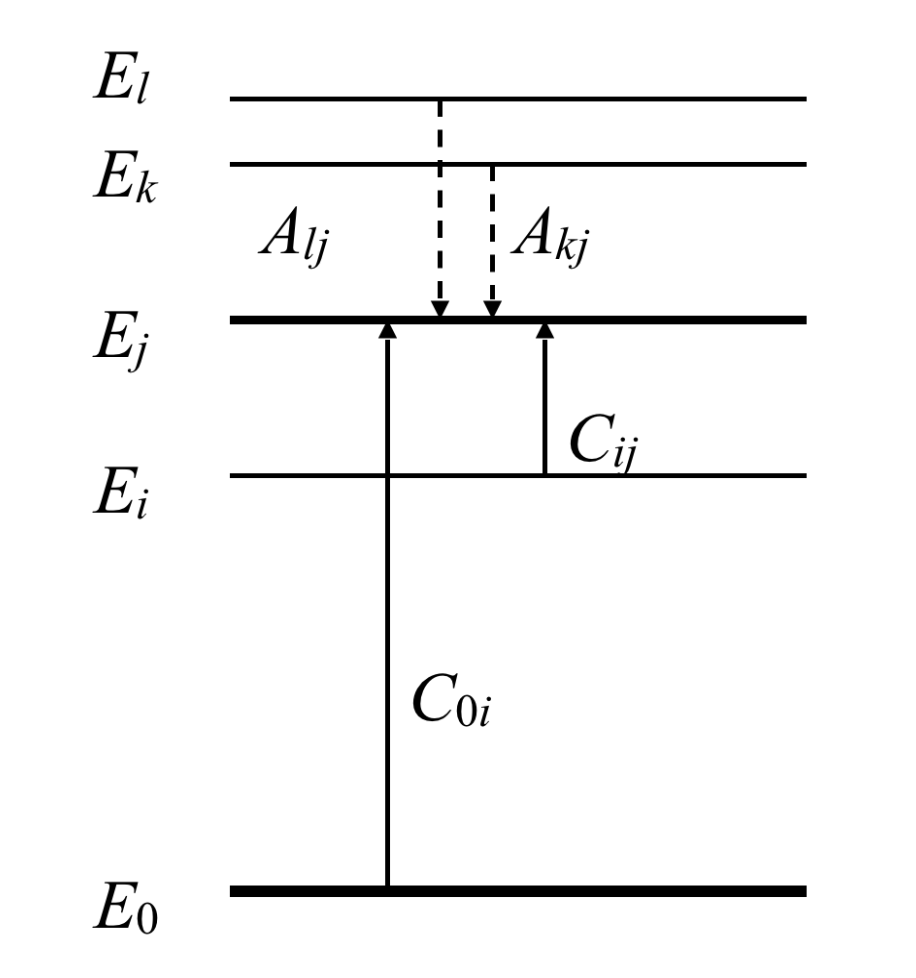
\includegraphics[width=0.35\textwidth]{figures/fig11a}
         }
         \hspace{0.05\columnwidth}
         \subfloat[\label{sub:fig11b}]{
           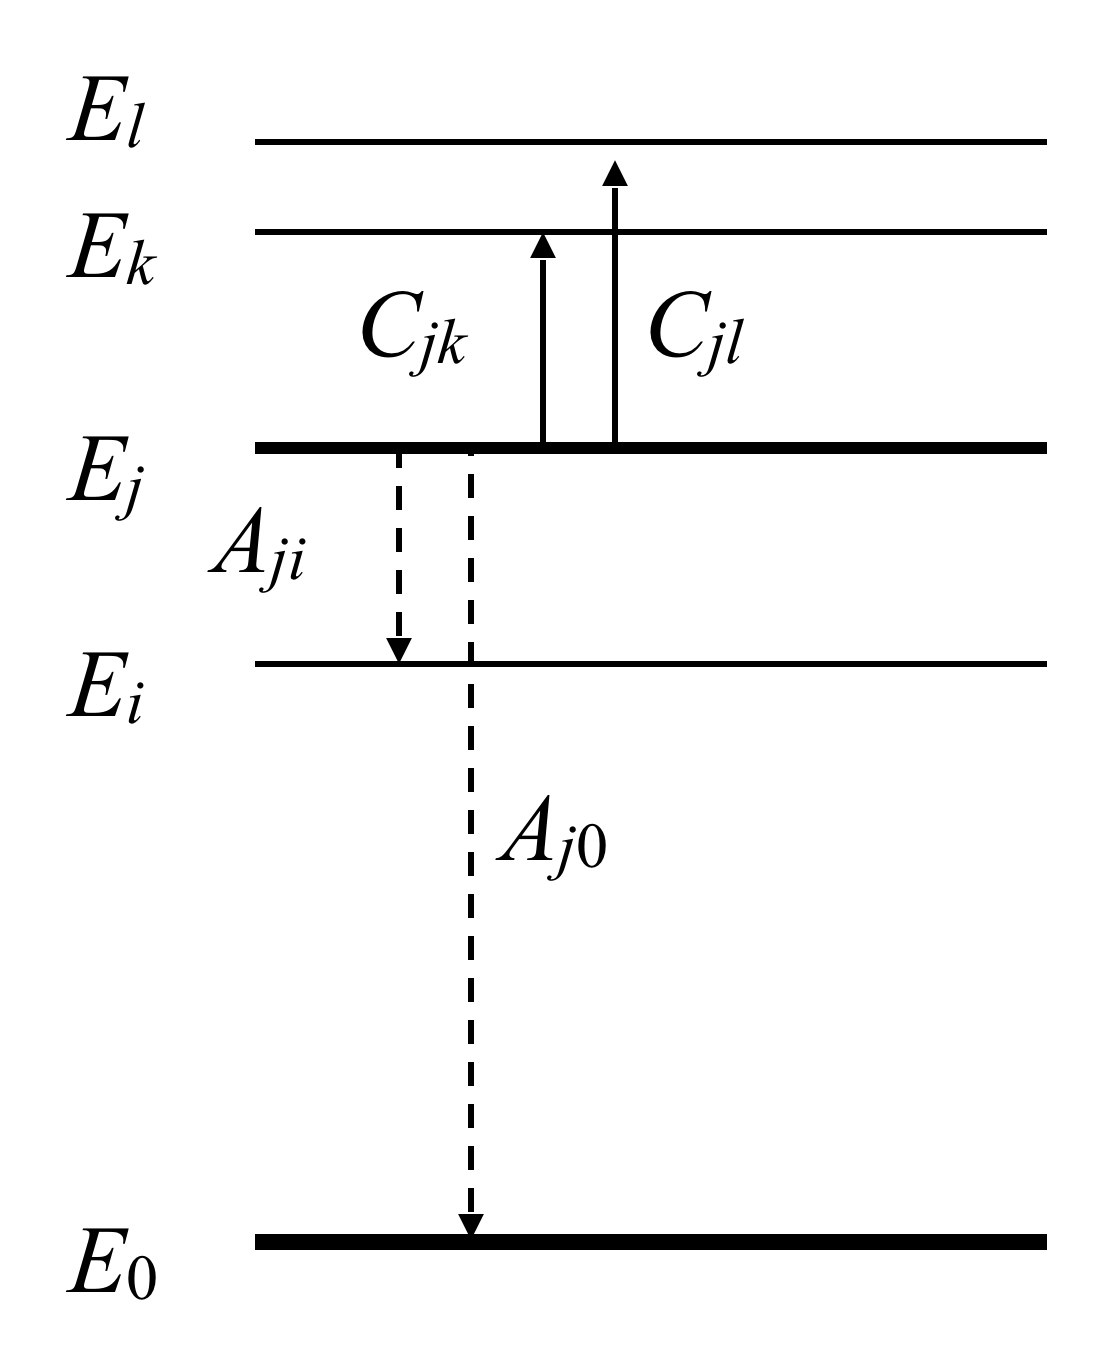
\includegraphics[width=0.305\textwidth]{figures/fig11b}
         }
         \caption{Схема основных процессов уровня: \pt(a) заселение, \pt(b) расселение.}
         \label{fig:fig11}
    \end{center}
\end{figure}

Населенность \math{N_j}$ уровня \math{E_j}$ в стационарном случае определяется балансом процессов его заселения
и расселения. Схема основных процессов заселения уровня \math{E_j}$ представлена на рис.~\ref{fig:fig11}~\subref{sub:fig11a}.
Основным процессом заселения рассматриваемого уровня \math{E_j}$ является его заселение прямым
электронным переходом с основного состояния \math{E_0}$ и с метастабильного \math{E_i}$.

Скорости процессов \math{C_{0j}}$ и \math{C_{ij}}$ определяются соотношениями:
\begin{equation}C_{0j} = \sqrt{2 \over m_e} \int_{E_j}^{\infty} \sigma_{0j}(E) f_e(E) \sqrt{E} dE\end{equation}
и
\begin{equation}C_{ij} = \sqrt{2 \over m_e} \int_{E_j - E_i}^{\infty} \sigma_{ij}(E) f_e(E) \sqrt{E} dE\end{equation}
соответственно, где …

Сечения \math{\sigma_{0j}(E)}$ и \math{\sigma_{ij}(E)}$ расчетные и экспериментальные, можно найти в литературе
или базе данных NIST [ССЫЛКА НА ИСТОЧНИК]. Типичный вид сечений представлен на рис. \ref{fig:fig12}.
Что касается вида ФРЭ, то она сильно зависит от параметров плазмы. При высоких давлениях ФРЭ приближается
к максвелловской функции. Однако, при низких давлениях плазма сильно неравновесна, и вид функции ФРЭ должен
быть определен дополнительными методами. Кроме столкновительного заселения уровень \math{E_j}$ заселяется
также путем радиационного распада верхних \math{k}$-уровней \math{E_k~>~E_j}$ cо скоростью \math{A_{kj}}$ при \math{k > j}$.
Значения \math{A_{kj}}$ также табулированы в базе данных NIST.
\begin{figure}[t]
  \centering
  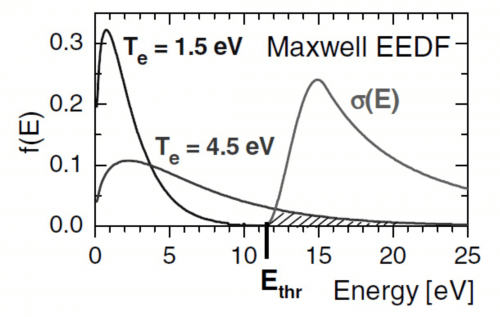
\includegraphics[width=8cm]{figures/fig12}
  \caption{Типичный вид сечения \math{\sigma}$ и максвелловской ФРЭ. \math{T_e}$ - температура электронов, \math{E_{thr}}$ - пороговая энергия..}
  \label{fig:fig12}
\end{figure}

Схема основных процессов расселения уровня \math{E_j}$ представлена на рис.~\ref{fig:fig11}~\subref{sub:fig11b}.
Этими процессами также являются явления спонтанного распада возбужденных уровней и столкновительные процессы,
индуцированные свободными электронами.

Приравняв скорости заселения и расселения уровня \math{E_j}$, мы получим уравнение относительно ФРЭ \math{f_e(E)}$.
Это уравнение является некорректной задачей и для ее решения необходимы дополнительные данные о виде ФРЭ.
Эти данные могут быть получены путем решения кинетического уравнения Больцмана для соответствующих условий.

\section{Уравнение Больцмана для ФРЭ в положительном столбе газового разряда постоянного тока.}

Газовые разряды представляют собой крайне неравновесную систему, в которой средняя энергия электронов (температура)
на два порядка превышает температуру газа. Функция распределения электронов (ФРЭ) характеризуется нагревом
электронов электромагнитными полями и столкновениями их с нейтральными атомами, почти во всех случаях это распределение
отклоняется от равновесного (Максвелловского). Решение кинетического уравнения Больцмана для ФРЭ является
важнейшей задачей для точного моделирования плазмы, так как многие явления невозможно правильно понять
без кинетического анализа. Уравнение Больцмана существенно можно упростить из-за большого различия масс электронов и атомов.
В силу данного различия, затухание энергии электронов в упругих столкновениях с атомами происходит гораздо медленнее,
чем затухание импульса электронов (\math{m_e \ll M_a}$). Как следствие, ФРЭ в скоростном пространстве может быть представлена как сумма
большой изотропной \math{f_0}$ и малой анизотропной частей \math{f_1}$.

Выделяют три существенно различных случая. Первый случай, когда величины \math{P L \gg 1}$ и \math{{E P} \ll 1}$, где
\math{P}$ - давление газа, \math{L}$ - характерный размер плазмы, \math{E}$ - электрическое поле, а
пространственные градиенты \math{f_0}$ и \math{f_1}$ малы и определены локальными значениями электрического поля,
электронной плотности и составом плазмы. Тогда электроны могут быть описаны уравнениями жидкости с коэффициентами переноса,
полученными из локальной (не Максвелловской) ФРЭ. Обычно через уравнение Больцмана решают задачу нахождения
коэффициентов переноса и скоростей протекания реакции для данного приближения.

Второй случай соответствует столкновительной плазме, где характерный размер плазмы \math{L}$ значительно больше средней длины
свободного пробега электронов \math{\lambda}$, но сравним с длиной релаксации энергии электрона \math{\lambda_\epsilon}$.
В этом нелокальном режиме изотропная часть ФРЭ \math{f_0}$ в заданной точке зависит не только от электрических полей в этой точке,
но и от свойств плазмы в окрестности точки размера (эффект памяти), а анизотропная часть \math{f_1}$ является лишь функцией
электрического поля \math{E}$. В этом столкновительном режиме плазма не может быть описана гидродинамикой.

В третьем случае, при дальнейшем уменьшении \math{P L}$, средняя длина свободного пробега электрона будет сравнима c характерным размером плазмы
(\math{\lambda \sim L)$. В этом почти бесстолкновительном случае анизотропная часть в точке определяется не только
значением напряженности электрического поля в этой точке, но и профилем электрического поля вдоль траектории электрона.
В результате локальная зависимость между плотностью тока и электрическим полем (закон Ома) становится недействительной \cite{Kolobov}.

Плазма тлеющего разряда низкого давления имеет сильно неравновесный характер. Рождение заряженных частиц происходит
преимущественно в объемных процессах, а гибель на стенках разрядной камеры. Энергию электроны приобретают,
разгоняясь в электрическом поле, а теряют в упругих и неупругих столкновениях. Количественное описание этих процессов
возможно только на кинетическом уровне \cite{Zobnin}.

В данной работе положительный столб газового разряда находится под низким давлением порядка 60~Па и имеет диаметр трубки 30~мм (см. раздел \ref{sec:sec_31}),
а значит для описания кинетических процессов с помощью уравнения Больцмана необходимо пользоваться почти бесстолкновительным приближением.

Кинетическое уравнение Больцмана представляет собой интегродифференциальное уравнение, описывающее эволюцию функции
распределения частиц в шестимерном (6-D) фазовом пространстве. Данное уравнение было выведено Людвигом Больцманом в 1872 г.
Оно до сих пор остается основой кинетической теории газов и оказывается плодотворным не только для исследования
классических газов, которые имел в виду Больцман, но - при соответствующем обращении - и для излучения переноса
электронов в твердых телах и плазме \cite{Cherchin'yani}. В общем виде оно выглядит следующим образом (также данное
уравнение называют уравнением Власова):

\begin{equation}
    {\partial f_e \over \partial t} + (\vec{v}, \vec{\Delta}_r) f_e + (\vec{a}, \vec{\Delta}_v) f_e = I
    \label{eq:vlasov}
\end{equation}
где \math{f_e = f_e(\vec{r}, \vec{v}, t)}$~--~функция распределения электронов,
\math{\vec{r}}$~--~вектор положения в физическом пространстве, \math{\vec{v}}$~--~вектор скорости,
\math{\vec{a}}$~--~вектор ускорения, \math{t}$~--~время, \math{I}$~--~интеграл столкновений,
является интегральным оператором в пространстве скоростей, в котором должны быть учтены все элементарные процессы
с участием электронов, приводящие к изменению их числа в объеме \math{dx dy dz dv_x dv_y dv_z}$ фазового пространства.

Решение этого интегродифференциального нелинейного уравнения сопряжено с огромными математическими трудностями и
поэтому всегда проводится с привлечением ряда серьезных упрощений. Многие сотни журнальных публикаций посвящены
конкретным расчетам \math{f(V)}$ в различных условиях, однако среди них далеко не всегда удается найти требуемое.
Вместе с тем экспериментатору часто приходится хотя бы оценить ожидаемый вид \math{f(V)}$ в условиях его работы \cite{Kolesnikov}.

%{e \over m_e} \vec{E}

Для слабоионизированной плазмы столкновения электронов с нейтралами обычно преобладают над столкновениями между
заряженными частицами. Из-за разницы масс электрона и атома (\math{m_e \ll M_a}$) интеграл столкновения
для упругих взаимодействий электронов с тяжелыми нейтралами может быть записан в так называемой форме Лоренцевского газа
\cite{Kolobov}:
\begin{equation}
    I_{el} = - {1 \over v^2} {\partial \over \partial v} v^2 \Gamma - N v \int_{S^2} \sigma (v, |\Omega - \Omega^{'}|) [f(v, \Omega^{'}) - f(v, \Omega)] d \Omega
    \label{eq:lorentz}
\end{equation}
где \math{\Omega}$~--~телесный угол фазового пространства скоростей на единичной сфере \math{S^2}$ (\math{\vec{v} = v \Omega}$),
\math{\sigma}$~--~сечение столкновения, \math{N}$~--~концентрация атомов газа, поток \math{\Gamma}$ задается следующим образом:
\begin{equation}
    \Gamma = - {\delta \nu \over 2} \big{(} v f + {T \over m} {\partial f \over \partial v} \big{)}
\end{equation}
где \math{T}$~--~температура газа, \math{\nu}$~--~транспортная частота столкновений и \math{\delta = (2m / M)}$~--~
средняя доля энергии, которая теряется электронами в упругих столкновений. Первое слагаемое в (\ref{eq:lorentz}) мало, оно
отвечает за обмен энергиями между электронами и нейтралами. Второе слагаемое в (\ref{eq:lorentz}) описывает столкновения
электронов с бесконечно тяжелыми частицами, которые в основном не меняют свою энергию, а лишь изотропно меняют
распределение электронов. Таким образом для того, чтобы ФРЭ пришла в равновесие с полем необходимо, чтобы прошло время
намного превышающе \math{({\nu m / M})^{-1}}$ \cite{Tsendin}.

Таким образом, для почти бесстолкновительного случая в качестве приближения ФРЭ для решения уравнения Власова (\ref{eq:vlasov}) можно
использовать достаточно распространенное двухчленное приближение:
\begin{equation}f_e(\vec{r}, \vec{v}, t) = f_0(\vec{r}, \vec{v}, t) + { \vec{v} \over v} \vec{f_1} (\vec{r}, \vec{v}, t)\end{equation}
где \math{f_1}$ отвечает за анизотропию.

Подставив это приближение в уравнение (\ref{eq:vlasov}) и усреднив по направлениям скоростей (в силу их изотропности из-за
столкновений с тяжелыми частицами), получим следующую систему уравнений, которую называют системой
Давыдова-Эллиса \cite{Kolobov}:
\begin{equation}
 \begin{cases}
  {\partial \vec{f_1} \over \partial t} + \nu \vec{f_1} = - v \nabla f_0 - {e \vec{E} \over m} {\partial f_0 \over \partial v},
   \\
   {\partial f_0 \over \partial t} + {v \over 3} div(\vec{f_1}) + {1 \over 3v^2} {\partial \over \partial v } ({ v^2 e \vec{E} \over m} \vec{f_1} ) = S_0
 \end{cases}
 \label{eq:davydov-ellis}
\end{equation}
Здесь \math{e}$~--~модуль заряда электрона, \math{m}$~--~масса электрона, \math{S_0}$ —  часть интеграла столкновений,
отвечающая за упругие и неупругие электрон-атомные столкновения и электрон-электронные взаимодействия

В левой части первого уравнения системы (\ref{eq:davydov-ellis}) можно пренебречь слагаемым
{\partial \vec{f_1} \over \partial t}$, так как мы рассматриваем выход ФРЭ на стационарный уровень во времени,
где анизотропические эффекты уже не имеют значения.

Перейдя от скоростей к энергиям \math{v = \sqrt{2 \epsilon \over m}}$,
\math{{\partial f(v) \over \partial v}  = {\partial f(\epsilon) \over \partial \epsilon} \sqrt{2 \epsilon m}}$
в системе Давыдова-Эллиса (\ref{eq:davydov-ellis}) и подставив выражение для \math{\vec{f_1}}$ в нижнее уравнение, получим:
\begin{equation}
    \begin{gathered}
        \sqrt{\epsilon} {\partial f_0 \over \partial t} = \sqrt{2 \over m} \big{[} S_0 + {\partial \over \partial \epsilon}
        [\epsilon^{3 \over 2} ({2 m \over M} \nu f_0 + {e^2 (\vec{E}, \vec{E}) \over 3 \nu} {\partial f_0 \over \partial \epsilon})] \big{]}
    \end{gathered}
\end{equation}
где \math{M}$ - масса молекулы неона.

Поскольку столб газового разряда геометрически представляет собой продольную трубку,
вдоль которой течет ток, то модуль электрического поля равен продольной составляющей \math{|\vec{E}|} = E_z}$, также его
называют осевым электрическим полем. Подставив значение транспортной частоты \math{\nu = N_g \sigma_t \sqrt{\epsilon}}$ и
осевого электрического поля, а также выполнив незначительные преобразования (в том числе переобозначение \math{f_0 = f}$), получим:
\begin{equation}
    \begin{gathered}
        \sqrt{\epsilon} {\partial f \over \partial t } = \sqrt{2 \over m} \big{[} S_0 + 2 {m \over M} N_g
        {\partial \over \partial \epsilon} \big{[} \sigma_t \epsilon^2 f \big{]}
        + {e^2 E_z^2 \over 3 N_g} {\partial \over \partial \epsilon} \big{[} {\epsilon \over \sigma_t}
        {\partial f \over \partial \epsilon} \big{]} \big{]}
    \end{gathered}
    \label{eq:main_eq}
\end{equation}

Вид \math{S_0}$ зависит от того, какие взаимодействия с электронами учитываются.
В данной работе использовался следующий вид \math{S_0}$, записанный в дискретной форме:
\begin{equation}
    S_0 = \sum_k \big{[} \sqrt{\epsilon + \epsilon_k} \nu_k (\epsilon + \epsilon_k)f(\epsilon + \epsilon_k) - \sqrt{\epsilon} \nu_k(\epsilon)f(\epsilon) \big{]}
    \label{eq:S_0}
\end{equation}
суммирование проводится по всем верхним энергетическим уровням k, которые больше аргумента функции \math{\epsilon}$,
частота столкновения k-уровня записывается так \math{\nu_k(\epsilon) = \sigma_k(\epsilon)N_g\sqrt{\epsilon}}$,
\math{N_g}$ - концентрация атомов.

В почти бесстолкновительном случае для поиска концентрации атомов Ne \math{N_g}$ можно воспользоваться уравнением состояния идеального газа,
поскольку атомы между собой почти не взаимодействуют:
\begin{equation}
    N_g = {P \over k_b T}
    \label{eq:concentration}
\end{equation}
где \math{P}$~--~давление газа 60~Па; \math{k_b}$~--~постоянная Больцмана; \math{T}$~--~температура газа 294~K.

\section{Решение уравнения Больцмана и результаты}

В данном подразделе описываются численные подходы, алгоритмы и аппроксимации необходимые для нахождения численного решения
функций распределения электронов для различных осевых электрических полей в диапазоне \math{1 \le E_z \le 10}$~В/см,
которые задаются параметрически.

Рассматривается задача решения разностной схемы относительно \math{f}$ на основе уравнений (\ref{eq:main_eq}) и (\ref{eq:S_0}).
Данная задача является краевой: вероятность нахождения электронов при бесконечно большой энергии стремится к нулю, а
вероятность нахождения электронов с положительном энергией максимальна, т.е. первая производная ФРЭ по энергии в нуле
будет равна нулю. Имеем следующие граничные условия:
\begin{equation}
    \begin{cases}
        {d f \over d \epsilon}(0) = 0
        \\
        f(\infty) = 0
    \end{cases}
    \label{eq:borders}
\end{equation}

Если обратить внимание на уравнения (\ref{eq:main_eq}) и (\ref{eq:S_0}), то становится ясно, что аналитически выразить
\math{f}$ для явного построения разностной схемы невозможно, поскольку в (\ref{eq:S_0}) \math{f}$ принимает значения для
аргументов, отличных от \math{\epsilon}$. Следовательно, при данной трактовки задачи необходимо получить дополнительное граничное
условие для каждого элемента суммирования \math{\epsilon_k}$, например с помощью двухточечной краевой задачи (метод стрельбы),
и сводить исходную задачу к задаче Коши. Это довольно сложный подход, более того, нет необходимости для каждого момента времени
решать задачу Коши, поскольку нас интересует ФРЭ при выходе на стационарный уровень во времени, а не при сложных переходных процессах.

Предполагается, что функция распределения электронов при заданном электрическом поле выйдет на стационарый уровень: из-за
невысоких полей данное предположение более, чем разумно. Поэтому будем высчитывать с помощью метода временной эволюции
относительную разницу ФРЭ между итерациями по времени и смотреть, если относительное изменение достаточно незначительно, то ФРЭ вышла
на стационарный уровень; далее решается краевая задача с граничными условиями (\ref{eq:borders}).
Построим разностную схему для данного подхода:
\begin{equation}
\begin{small}
    \begin{gathered}
        f^n(\epsilon) = f^{n-1}(\epsilon) + \Delta t \sqrt{2 \over m \cdot \epsilon}
        \Big{[} N_g \sum_k
            \big{[}
                F^{n-1}_k (\epsilon + \epsilon_k) - F^{n-1}_k (\epsilon)
            \big{]} + \\
        {2 m N_g \over M}
            \big{[}
                {F^{n-1}_t(\epsilon + \Delta \epsilon) \cdot (\epsilon + \Delta \epsilon) -
                F^{n-1}_t(\epsilon - \Delta \epsilon) \cdot (\epsilon - \Delta \epsilon)  \over 2 \Delta \epsilon }
            \big{]} + \\
        {1 \over \Delta \epsilon} \cdot {e^2 E_z^2 \over 3 N_g} \cdot
            \big{[}
                {\epsilon + { \Delta \epsilon \over 2 } \over  \sigma_t(\epsilon + { \Delta \epsilon \over 2 })} \cdot
                {f^{n-1}(\epsilon + \Delta \epsilon) - f^{n-1}(\epsilon) \over \Delta \epsilon } -
                {\epsilon - { \Delta \epsilon \over 2 } \over  \sigma_t(\epsilon - { \Delta \epsilon \over 2 })} \cdot
                {f^{n-1}(\epsilon) - f^{n-1}(\epsilon - \Delta \epsilon) \over \Delta \epsilon }
            \big{]}
        \Big{]}
    \end{gathered}
\end{small}
\label{eq:razh_scheme}
\end{equation}
где \math{\epsilon}$~--~энергия в~эВ; \math{\Delta \epsilon}$~--~шаг по энергии в~эВ;
\math{f^n (\epsilon)}$~--~ФРЭ с энергией \math{\epsilon}$, имеющая \math{n}$-й шаг по времени;
\math{\sigma_t (\epsilon)}$~--~транспортное сечение упругого рассеяния;
\math{\sigma_k (\epsilon)}$~--~сечение неупругих столкновений для k-уровня;
\math{N_g}$~--~концентрация атомов \math{Ne}$ в см^{-3}; \math{M}$~--~масса молекулы Ne в граммах;
\math{m}$~--~масса электрона в граммах; \math{e}$~--~заряд электрона в Кл;
\math{k}$~--~итератор суммирования по всем энергиям верхних уровней, значения которых больше \math{\epsilon}$;
\math{E_z}$~--~осевое электрическое поле, которое задается параметрически в диапазоне \math{1 \le E_z \le 10}$~В/см с шагом \math{0.1}$~В/см;
для удобства записи выполнена замена
\math{F^n_i}(\epsilon) = f^n(\epsilon) \cdot \sigma_i(\epsilon) \cdot \epsilon }$, где \math{i}$ обозначает природу сечения.

\begin{figure}[t]
  \centering
  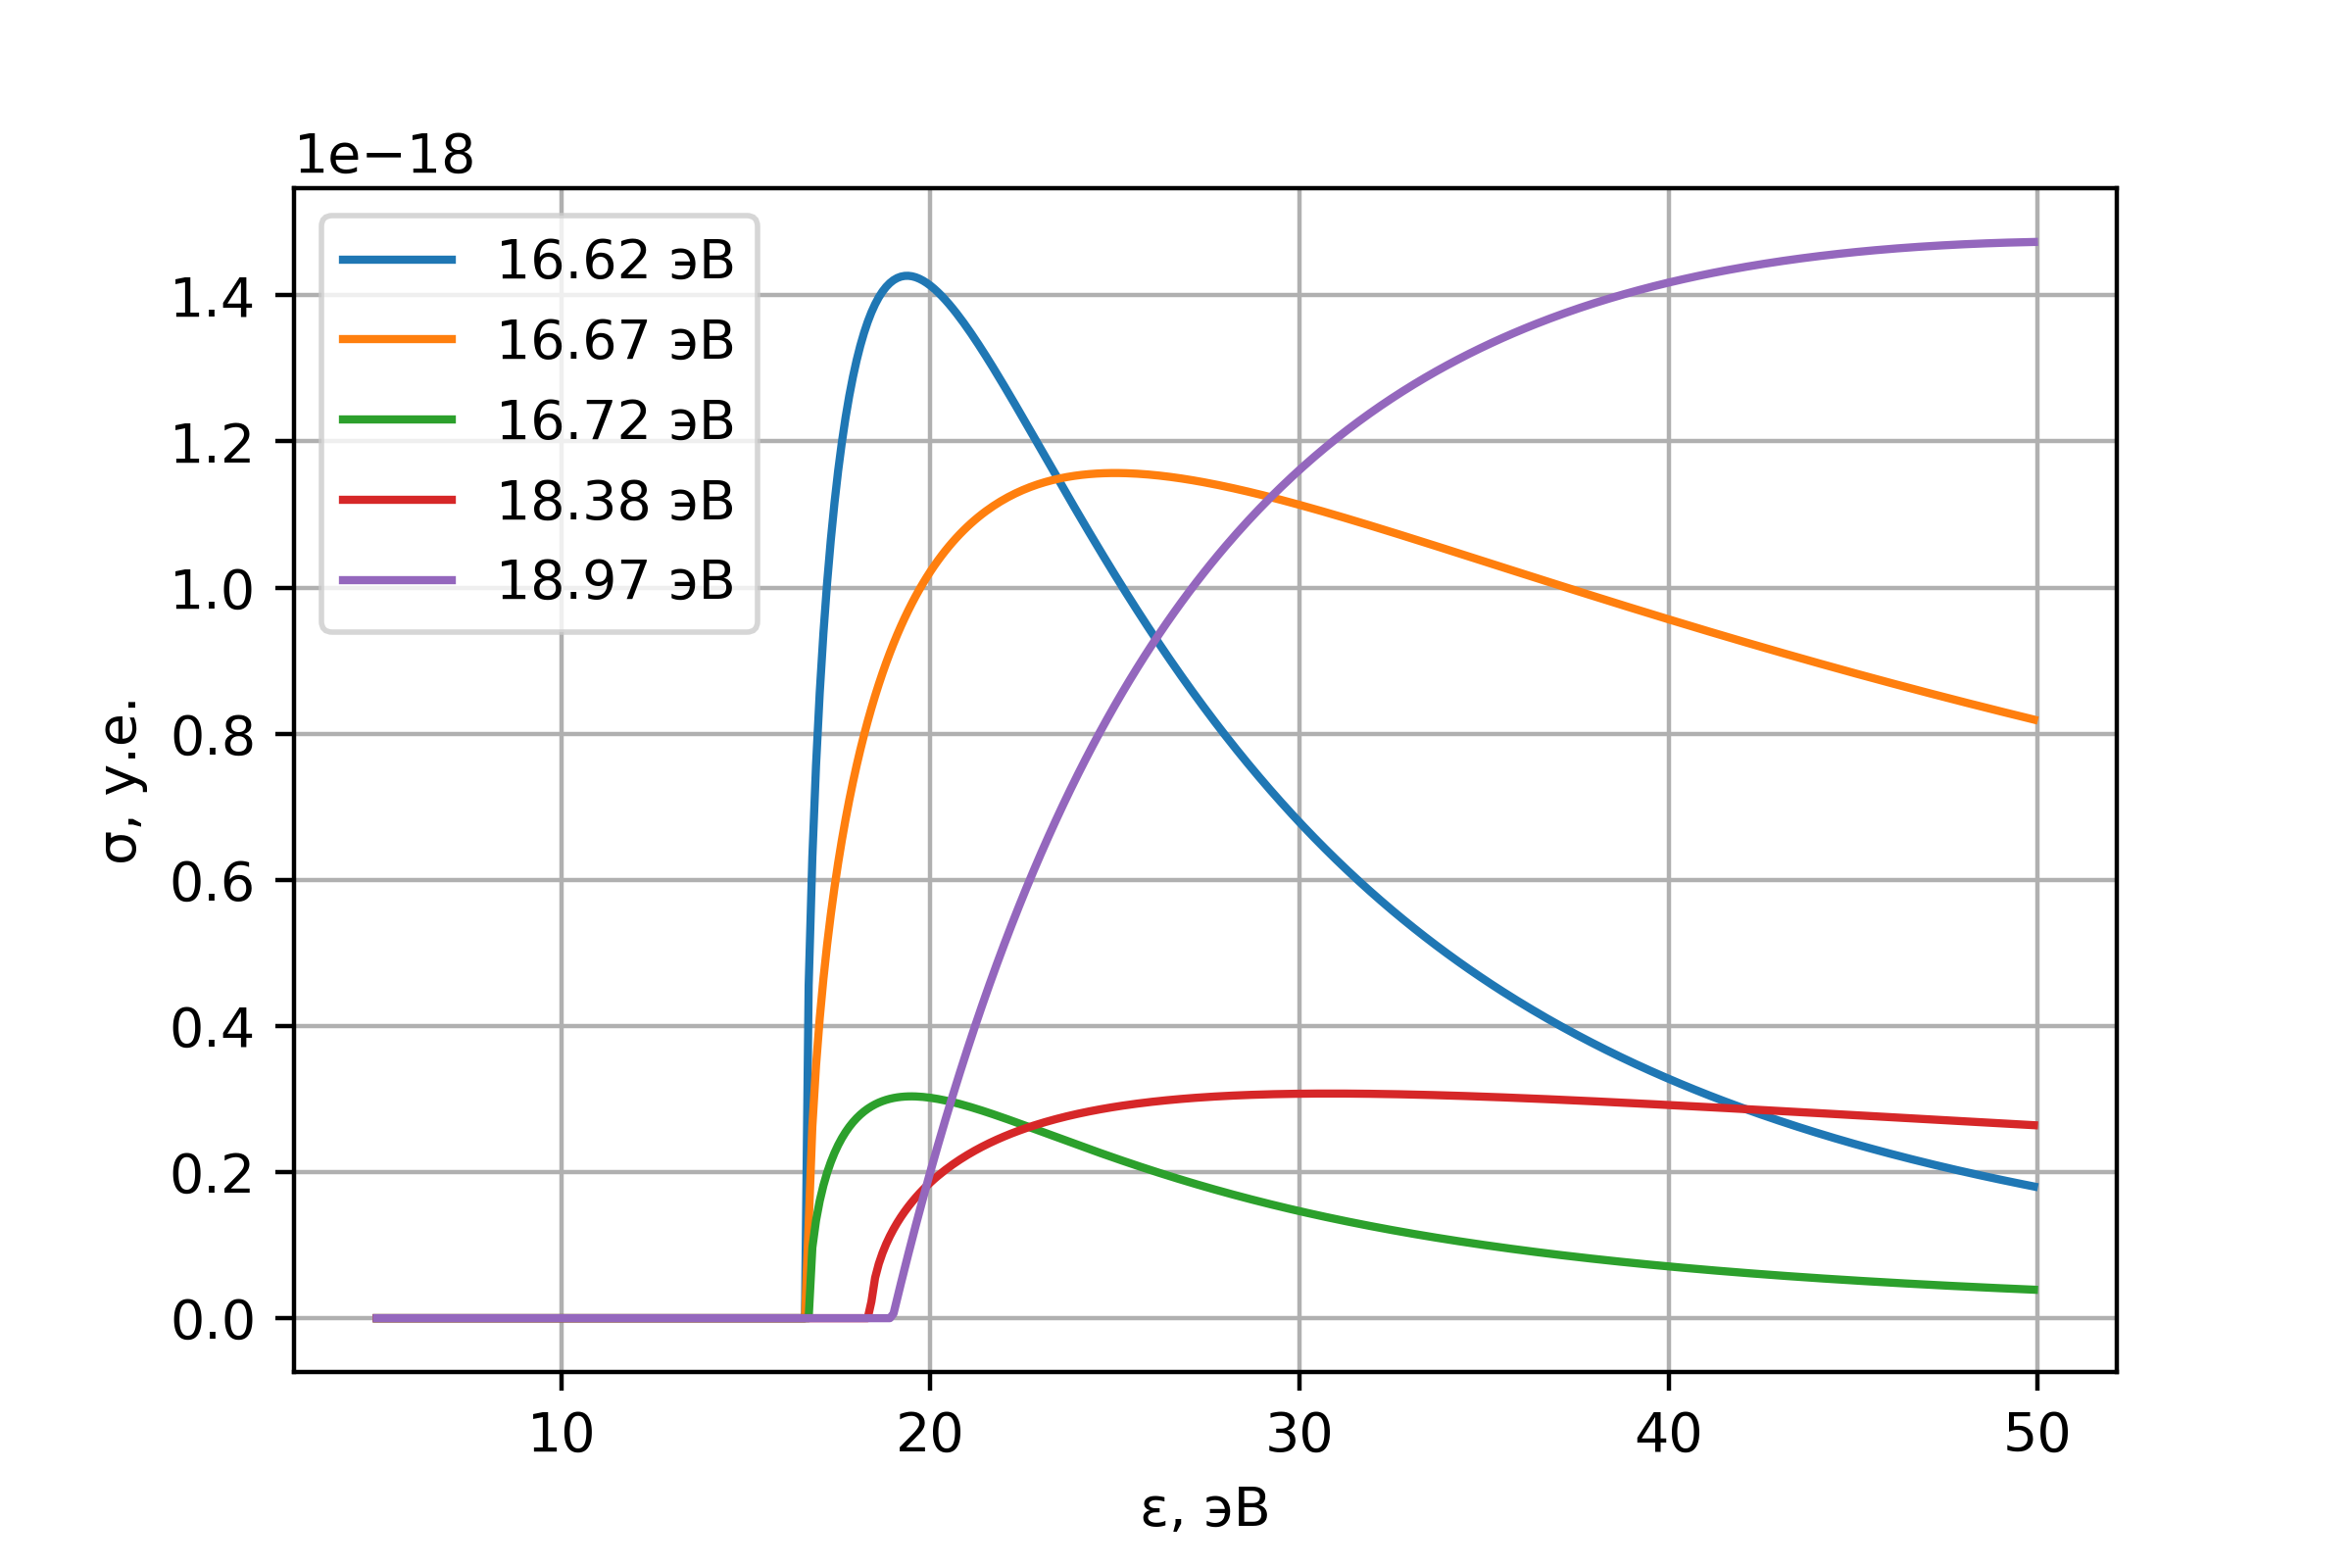
\includegraphics[width=15cm]{figures/fig13}
  \caption{Графическое представление некоторых аппроксимаций сечений рассеяния для различных энергетических уровней.}
  \label{fig:fig13}
\end{figure}

На языке разностной схемы граничные условия (\ref{eq:borders}) будут выглядить следующим образом:
\begin{equation}
    \begin{cases}
        f^n_0 = f^n_1
        \\
        f^{n}_K = 0
    \end{cases}
    \label{eq:razn_borders}
\end{equation}
где K~--~максимальное количество шагов по энергии, в рамках данной задачи энергию равной 50~эВ можно считать уже бесконечно большой.
То есть при шаге \math{\Delta \epsilon = 0.1}$~эВ максимальное количество шагов по энергии будет \math{K = 500}$.

В качестве начальных условий при \math{t = 0}$ для первого вычисления ФРЭ (при \math{E = 1}$~В/см) предлагается взять
распределение Больцмана:
\begin{equation}
    f^0 (\epsilon) = 0.7 \cdot e^{- {\epsilon \over 6}}
    \label{eq:start_condition}
\end{equation}

Данная функция намного ближе к итоговому решению, чем прямая, а значит для сходимости нужно будет выполнить меньше итераций
по времени: чем приближеннее возьмем начальное условие, тем быстрее наступит стационарный уровень. По данным соображениям
для подсчета ФРЭ для следующих полей удобнее всего брать за начальные условия результаты предыдущего расчета.

В данной работе использовались следующие аналитические аппроксимации для сечений элементарных процессов, полученные частично из
\cite{Zobnin}, частично из последних трудов Зобнина~А.~В.:
\begin{figure}[t]
  \centering
  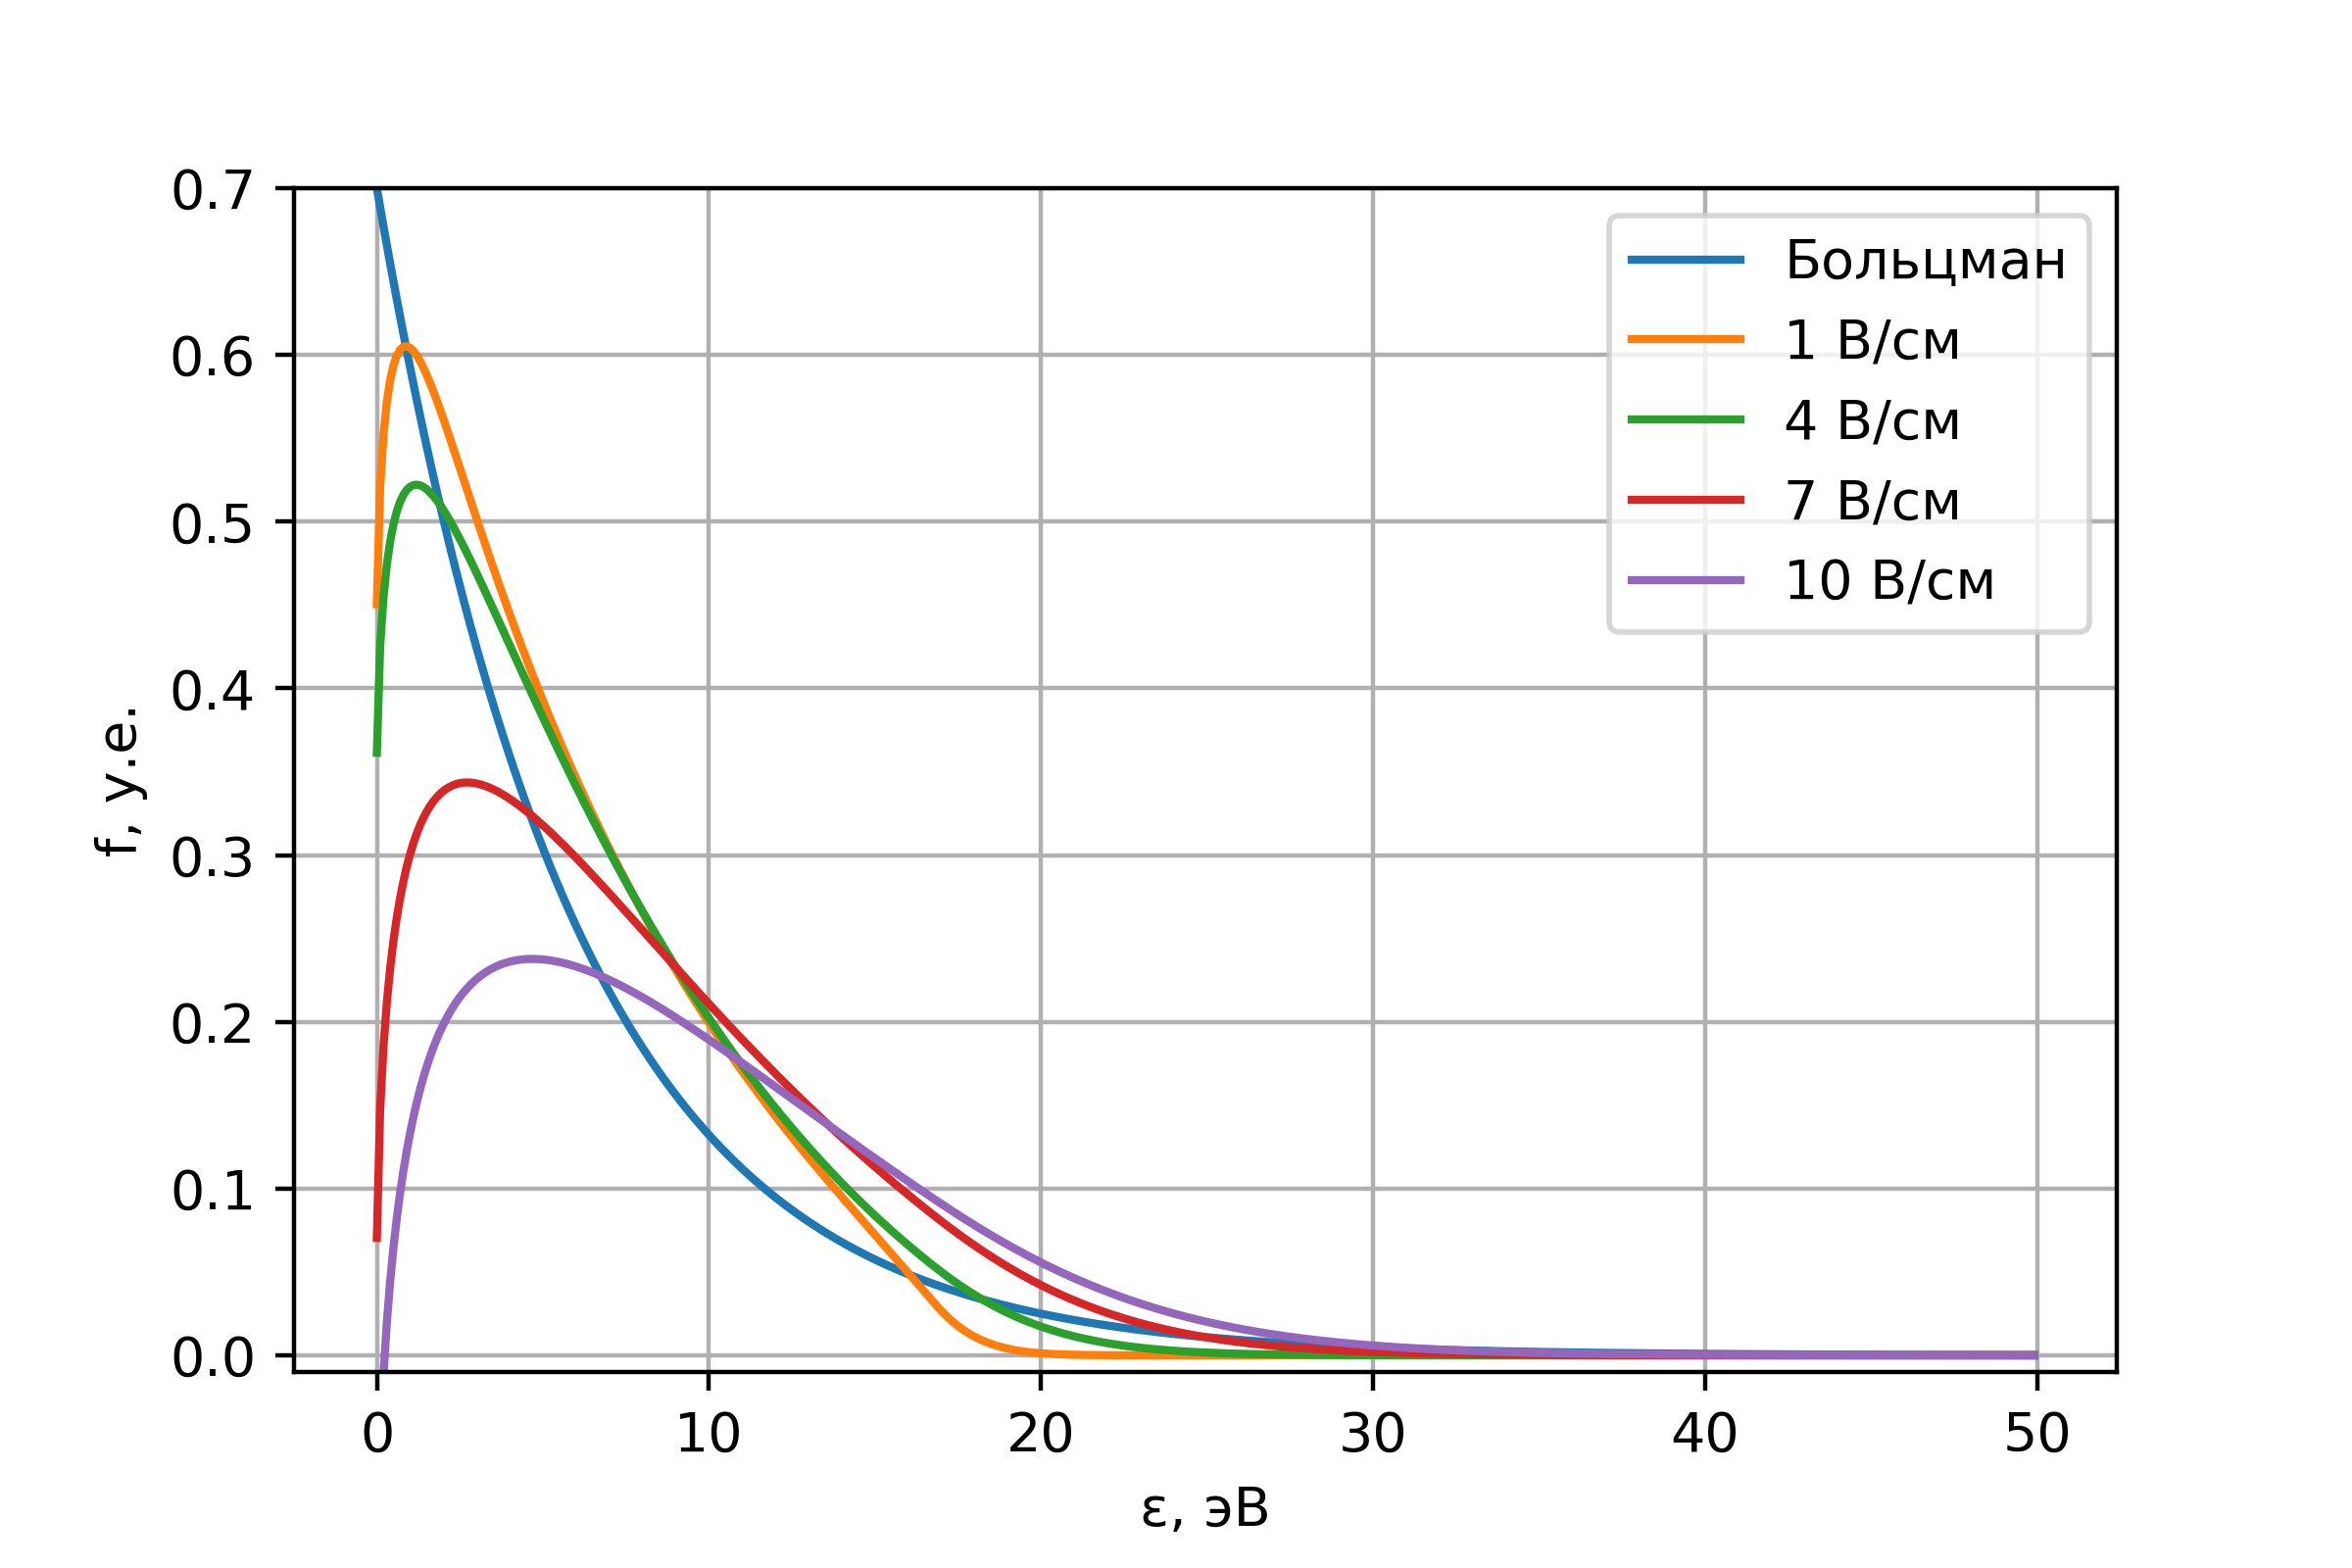
\includegraphics[width=15cm]{figures/fig14}
  \caption{Зависимость расчетной функции распределения электронов от энергии и осевого электрического поля,
  заданного параметрически для некоторых значений; также нанесено распределение Больцмана, которое использовалось в качестве
  начального условия (\ref{eq:start_condition}).}
  \label{fig:fig14}
\end{figure}
\begin{equation*}
    \sigma_t(\epsilon) = \begin{cases}
    \big{[}
        2.56 + 0.57 \cdot \ln
        \big{(}
            0.02 + {\epsilon \over 5.5 + \epsilon^2 } + {0.15 \cdot \epsilon^2 \over 12 + \epsilon + 3 \cdot 10^{-5} \cdot \epsilon^4}
        \big{)}
    \big{]} \cdot 10^{-16}, \epsilon > 0 \\
    \big{[}2.56 + 0.57 \cdot \ln(0.02)\big{]} \cdot 10^{-16}, \epsilon \le 0
    \end{cases}
\end{equation}
\begin{equation*}
    \sigma_{16.62}(\epsilon) = \begin{cases}
    {2.742 \cdot 10^{-14} \over \epsilon^3} \cdot \sqrt{\epsilon - 16.6 \over \epsilon}, \epsilon > 16.62 \\
    0, \epsilon \le 16.62
    \end{cases}
\end{equation}
\begin{equation*}
    \sigma_{16.67}(\epsilon) = \begin{cases}
    {5.01 \cdot 10^{-17} \over \epsilon} \cdot \sqrt{\epsilon - 16.67 \over \epsilon}, \epsilon > 16.67 \\
    0, \epsilon \le 16.67
    \end{cases}
\end{equation}
\begin{equation*}
    \sigma_{16.72}(\epsilon) = \begin{cases}
    {5.941 \cdot 10^{-15} \over \epsilon^3} \cdot \sqrt{\epsilon - 16.7 \over \epsilon}, \epsilon > 16.72 \\
    0, \epsilon \le 16.72
    \end{cases}
\end{equation}
\begin{equation*}
    \sigma_{16.85}(\epsilon) = \begin{cases}
    6 \cdot 10^{-18} \cdot \ln\big{(}{\epsilon \over 16.8}\big{)} + 5.7 \cdot 10^{-18} \sqrt{\epsilon - 16.8 \over \epsilon}, \epsilon > 16.85 \\
    0, \epsilon \le 16.85
    \end{cases}
\end{equation}
\begin{figure}[t]
    \begin{center}
         \subfloat[\label{sub:fig15a}]{
           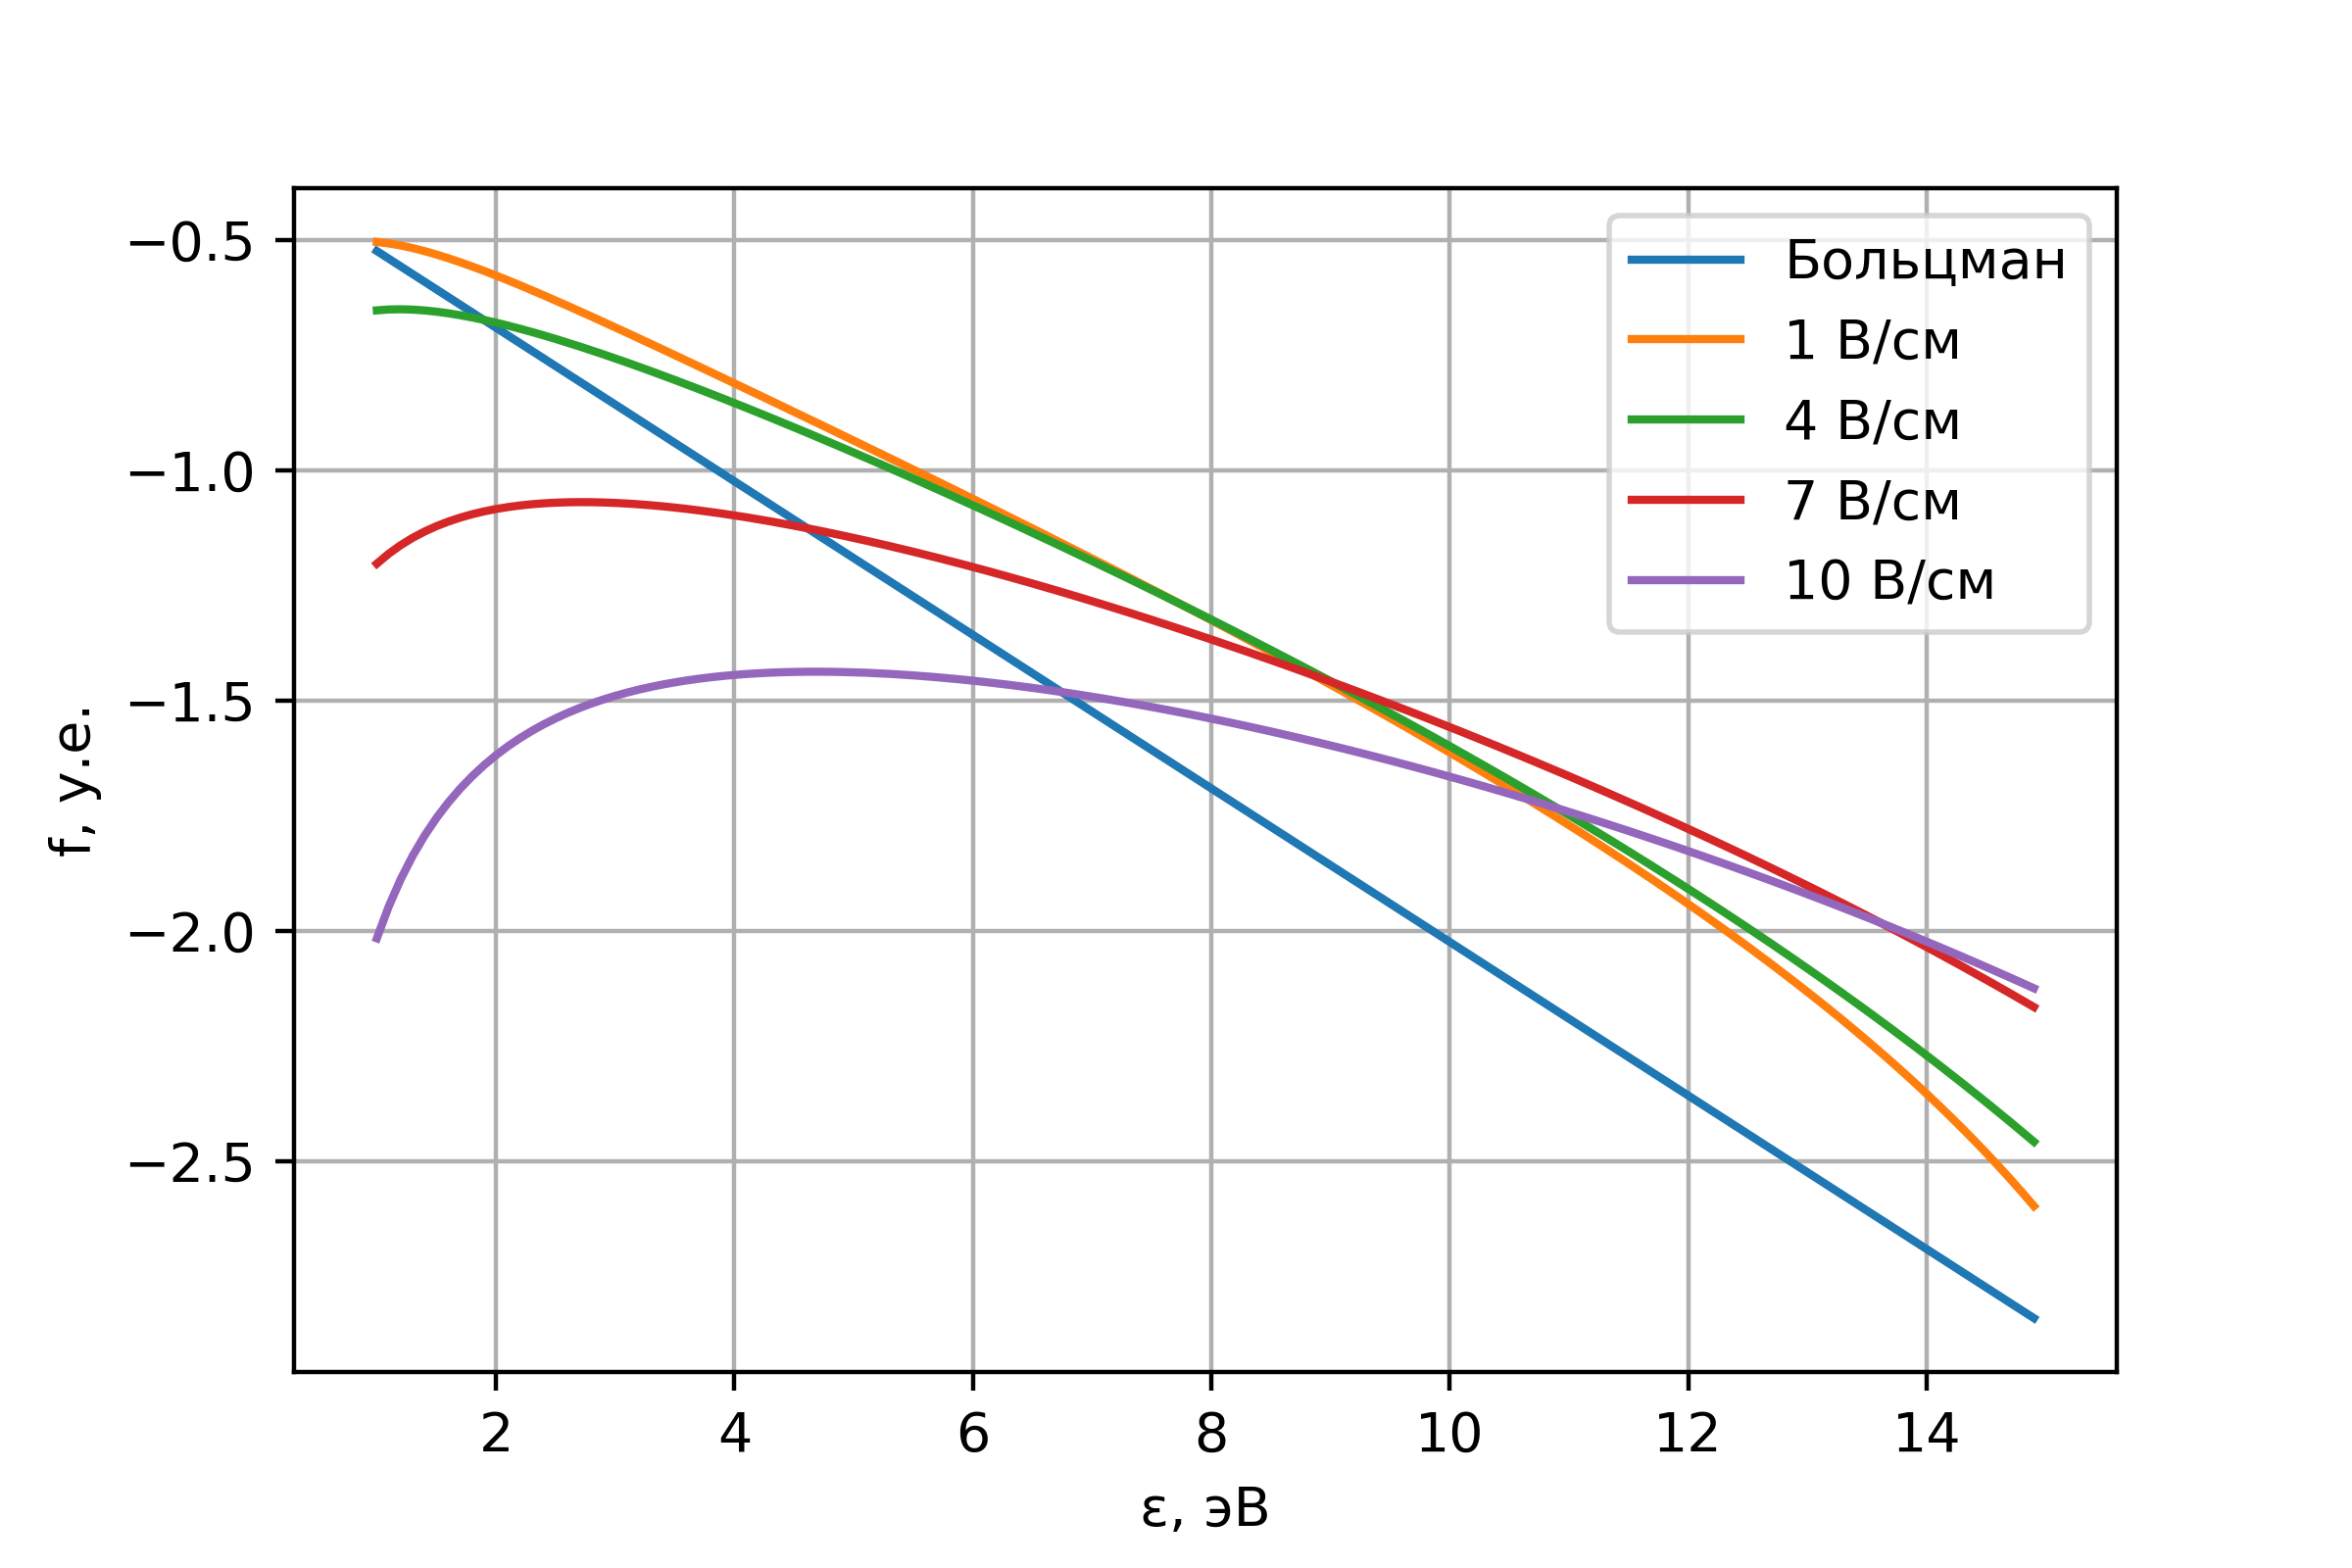
\includegraphics[width=0.49\textwidth]{figures/fig15a}
         }
         \subfloat[\label{sub:fig15b}]{
           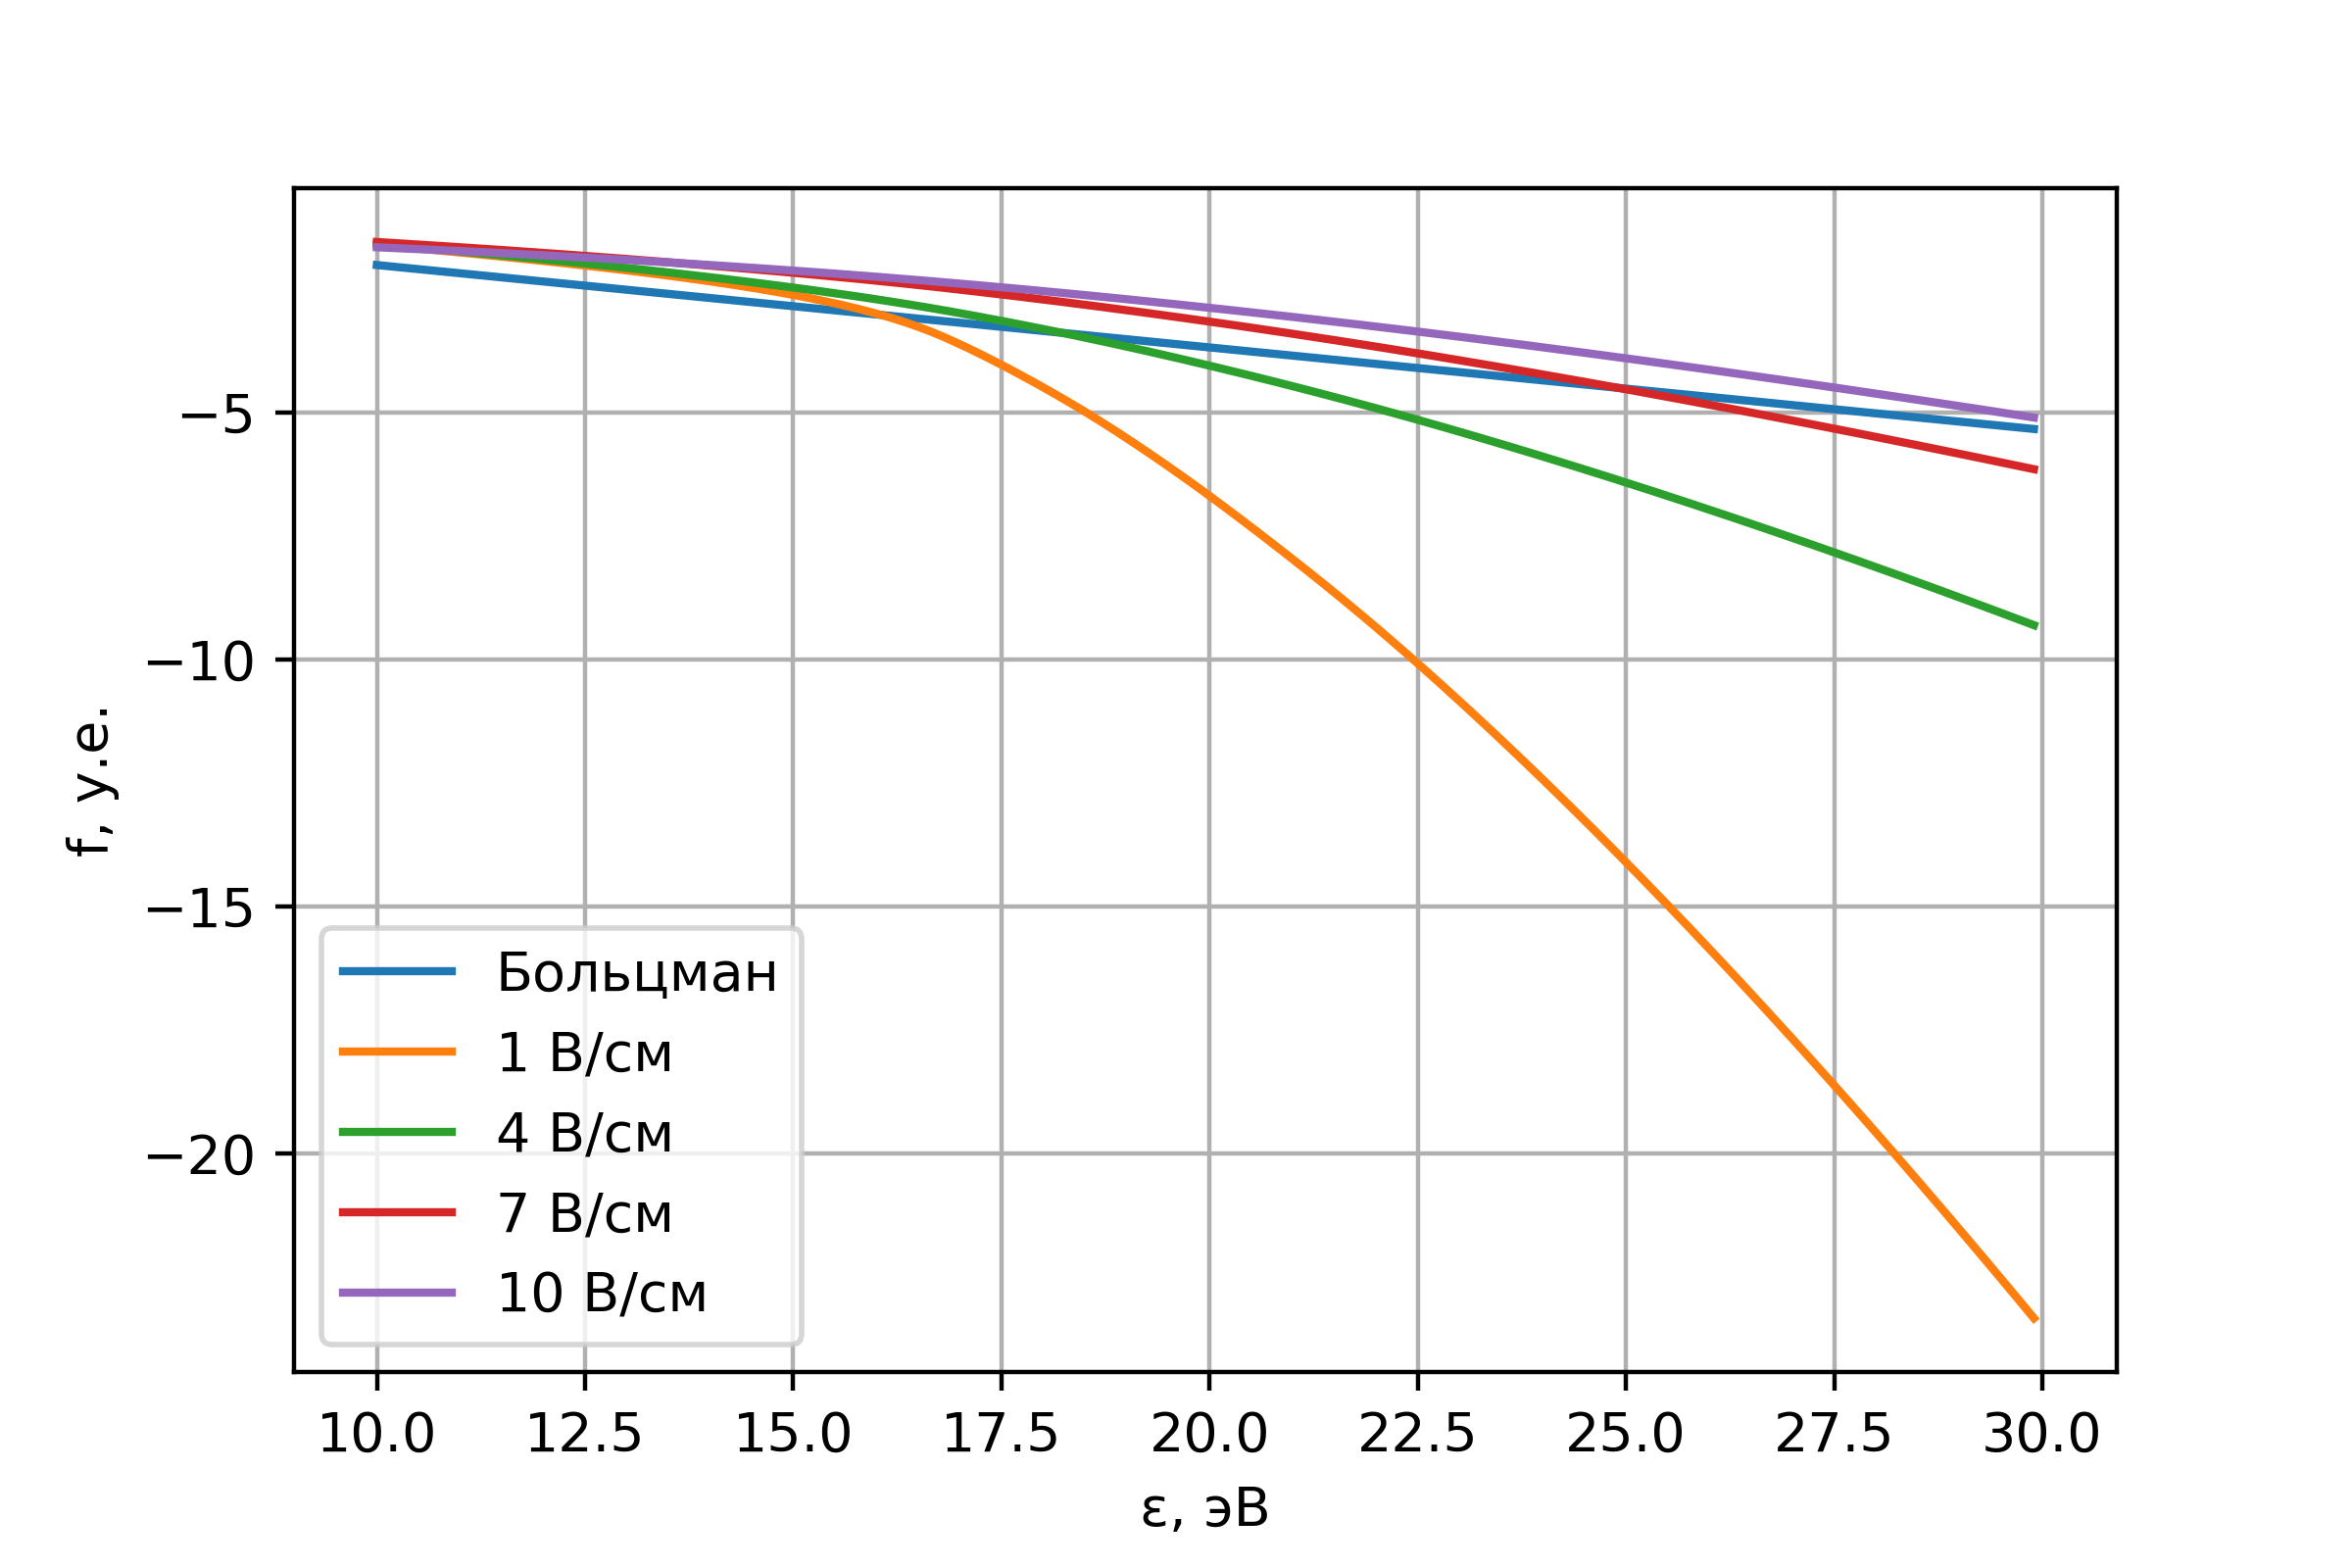
\includegraphics[width=0.49\textwidth]{figures/fig15b}
         }
         \caption{Зависимость расчетной функции распределения электронов от энергии и осевого электрического поля,
                  заданного параметрически для некоторых значений, в логарифмическом масштабе:
                  \pt(a) в диапазоне \math{1 \le \epsilon \le 15 }$~эВ, \pt(b) в диапазоне \math{10 \le \epsilon \le 30 }$~эВ;
                  также нанесено распределение Больцмана, которое использовалось в качестве начального условия (\ref{eq:start_condition}).

         }
         \label{fig:fig15}
    \end{center}
\end{figure}
\begin{equation*}
    \sigma_{18.38}(\epsilon) = \begin{cases}
    {2.024 \cdot 10^{-17} \over \epsilon + 11} \cdot \sqrt{\epsilon - 18.38 \over \epsilon}, \epsilon > 18.38 \\
    0, \epsilon \le 18.38
    \end{cases}
\end{equation}
\begin{equation*}
    \sigma_{18.6}(\epsilon) = \begin{cases}
    {1.44 \cdot 10^{-16} + 1.4 \cdot 10^{-18} \cdot \epsilon \over \epsilon + 50} \cdot \sqrt{\epsilon - 18.6 \over \epsilon}, \epsilon > 18.6 \\
    0, \epsilon \le 18.6
    \end{cases}
\end{equation}
\begin{equation*}
    \sigma_{18.71}(\epsilon) = \begin{cases}
    {3.461 \cdot 10^{-15} + 1.565 \cdot 10^{-16} \cdot \epsilon + 1.5 \cdot 10^{-18} \cdot \epsilon^2 \over (\epsilon + 37.4)(\epsilon + 27)} \cdot \sqrt{\epsilon - 18.7 \over \epsilon}, \epsilon > 18.71 \\
    0, \epsilon \le 18.71
    \end{cases}
\end{equation}
\begin{equation*}
    \sigma_{18.97}(\epsilon) = \begin{cases}
    {7.6 \cdot 10^{-17} \over \epsilon} \cdot \ln\big{(}{\epsilon \over 18.97}\big{)}, \epsilon > 18.97 \\
    0, \epsilon \le 18.97
    \end{cases}
\end{equation}
\begin{equation*}
    \sigma_{19.7}(\epsilon) = \begin{cases}
    1.8 \cdot 10^{-18} \cdot \sqrt{\epsilon - 19.7 \over \epsilon}, \epsilon > 19.7 \\
    0, \epsilon \le 19.7
    \end{cases}
\end{equation}
\begin{equation*}
    \sigma_{20.0}(\epsilon) = \begin{cases}
    1.5 \cdot 10^{-18} \cdot \sqrt{\epsilon - 20.0 \over \epsilon}, \epsilon > 20.0 \\
    0, \epsilon \le 20.0
    \end{cases}
\end{equation}
\begin{equation*}
    \sigma_{ion}(\epsilon) = \begin{cases}
    2.5 \cdot 10^{-17} \cdot {\epsilon - 21.5 \over 21.5}, \epsilon > 21.5 \\
    0, \epsilon \le 21.5
    \end{cases}
\end{equation}


Используя данные аппроксимации сечений, разностную схему, начальные и граничные условия (\ref{eq:razh_scheme}~--~\ref{eq:start_condition}),
итерационные шаги \math{\Delta \epsilon = 0.1}$~эВ и \math{\Delta t \sqrt{2 \over m} = 0.0002 }$~с~\math{\cdot}$~г^{\math{-{1 \over 2}}}$,
а также параметрически задавая осевое электрическое поле в диапазоне \math{1 \le E_z \le 10}$~эВ с шагом \math{\Delta E_z = 0.1}$~эВ,
рассчитаем ФРЭ. С графическим представлением некоторых результатов можно ознакомиться на рис. \ref{fig:fig14}.

Интенсивность свечения плазмы определенной длины волны формируется поведением ФРЭ при энергиях больше пороговой (до бесконечности),
которая имеет значение соответственно переходу для данной длины волны. Поэтому особый интерес в данной работе представляет
хвостовая часть полученной функции распределения электронов: в основном пороговая энергия для энергетических переходов неона больше
16~эВ. В обычном масштабе обнаружить на глаз поведение хвостовой части ФРЭ представляется невозможным (см.~рис~\ref{fig:fig14}):
хвостовая часть распределения Больцмана, как и остальных посчитанных распределений, сливаются между собой. Поэтому удобнее
всего перейти к логарифмическому масштабу ФРЭ (см.~рис~\ref{sub:fig15b}).


%\chapter{Влияние пылевых частиц на кинетические процессы}
\label{cha:ch_2}

\chapter{Космическая аппаратура “Плазменный кристалл-4”}
\label{cha:ch_3}
Космическая аппаратура “Плазменный~кристалл~-~4“ (КА~“ПК-4“) была введена в эксплуатацию на борту
Международной космической станции (МКС) в июне 2015~года. Установка предназначена для экспериментального
исследования пылевой плазмы в условиях микрогравитации. В отличие от предыдущей космической аппаратуры
“ПК-3” и “ПК-3~Плюс”, где пылевая плазма создавалась в емкостном радиочастотном (ВЧ) газовом разряде,
в КА~“ПК-4“ пылевая плазма создается в однородном положительном столбе газового разряда в режиме
комбинированного постоянного тока, а также в индуктивном ВЧ разряде. Условия микрогравитации оказывают
влияние на создание вытянутых пылевых облаков в однородном положительном столбе, благодаря чему становится возможным
создать в лабораторных условиях небольшое облако пыли со средним размером 1~см \cite{Usachev-Elbrus}.

\section{Экспериментальная установка}
\label{sec:sec_31}
\begin{figure}[t]
  \centering
  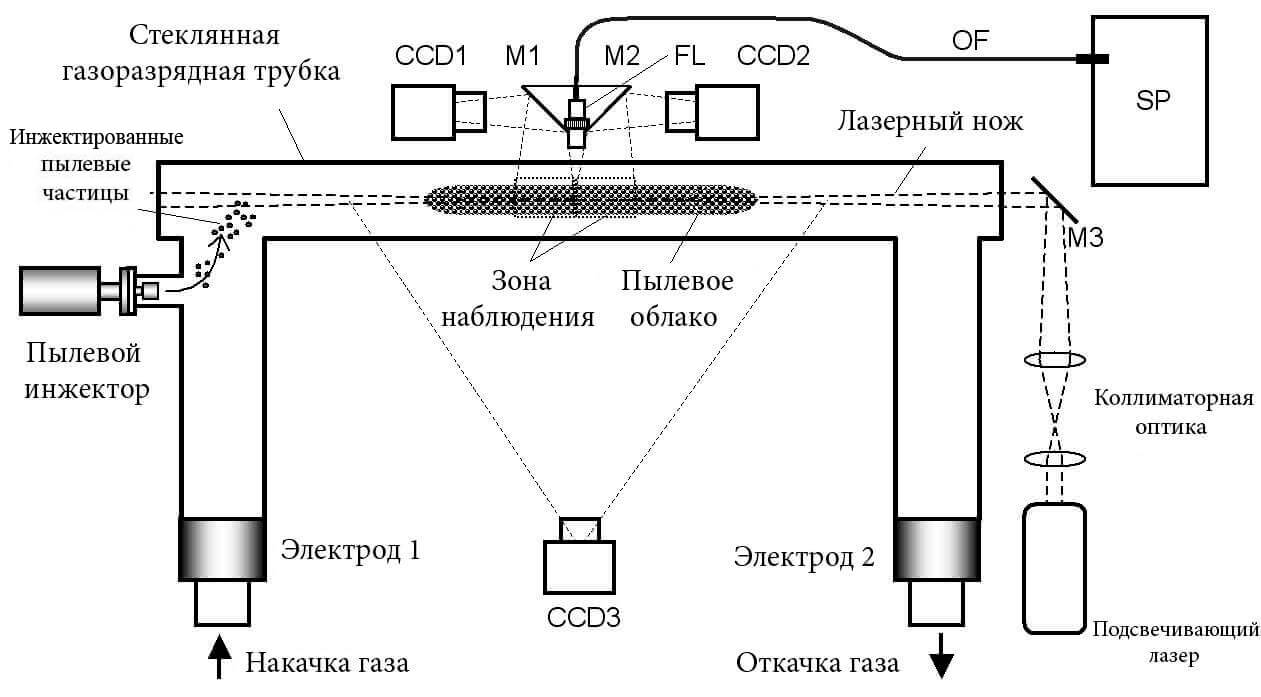
\includegraphics[width=12cm]{figures/fig31}
  \caption{Схема экспериментальной установки космической аппаратуры “Плазменный~кристалл-4”. Здесь CCD1,~CCD2~--~камеры высокого разрешения;
           M1,~M2,~M3~--~зеркала; OF~--~оптоволоконный кабель; SP~--~спектрометр.}
  \label{fig:fig31}
\end{figure}
Основой экспериментальной установки является П-образная стеклянная разрядная трубка с внутренним диаметром 30~мм
и общей длиной 85~см, которая заполнена молекулярным неоном под давлением 60~Па.
На концах трубки установлены цилиндрические электроды из нержавеющей стали, которые используются для создания
и поддержания разряда постоянного тока. Системы вакуумной откачки и накачки газа соединяются с концами трубки
через данные электроды. Прежде, чем трубка заполняется газом, в течение 2~дней она откачивается до давления высокого вакуума порядка \math{< 2 × 10^{-3}}$~Па, а
затем заполняется неоном до рабочего давления разряда порядка 60~Па. Ток разряда составляет \math{I_{DC} = 1}$~мА.

После заполнения рабочим газом, с катодной стороны разрядной трубки с помощью пылевого инжектора впрыскиваются
монодисперсные пластические (меламиноформальдегидные) микросферы (частицы пыли) с диаметром \marh{d~=~3.38 ± 0.07}~мкм,
которые, заряжаясь отрицательно, с помощью электрического поля постоянного тока, образуюшегося между катодом и анодом,
транспортируются в центр трубки для дальнейшего наблюдения. Пылевые частицы подсвечиваются зеленым
(532~нм) лазерным «ножом» и регистрируются двумя камерами наблюдения высокого разрешения (CCD1 и CCD2).
Для отслеживания макро поведения подсвеченной плазмы используется общая камера наблюдения (CCD3) (см~рис.~\ref{fig:fig31}).

Каждая камера CCD1/CCD2 имеет поле зрения \math{22 × 17}$~мм\math{^2}$, разрешение \math{1600 × 1200}$~пикселей, а также
частоту кадросмен 35~кадров в секунду. Камеры дополняют друг друга, присоединяясь меньшими сторонами и имеют общий размер
\math{44 × 17}$~мм\math{^2}$. Эффективная полуширина лазерного «ножа» составляет 50~мкм в центре поля зрения,
а также 180~мкм по краям.

Камера CCD3 имеет возможность просматривать всю трубку целиком c разрешением \math{640 × 480}$~пикселей
и частотой 15~кадров в секунду. Используя калейдоскопическую систему, камера CCD3 также наблюдает плазменное свечение
в центральной части разрядной трубки через 3~спектральных фильтра: один серый фильтр с пропусканием 12\% и два узкополосных
помеховых фильтров, настроенных на 705 и 587~нм.

Одна из копий модифицированной экспериментальной установки КА~“ПК-4“, которая в собранном виде  внешне не имеет существенных отличий,
находится в институте ОИВТ РАН (см~рис.~\ref{sub:photo-pk4}).

\begin{figure}[t]
    \begin{center}
         \subfloat[\label{sub:3D-scheme-pk4}]{
           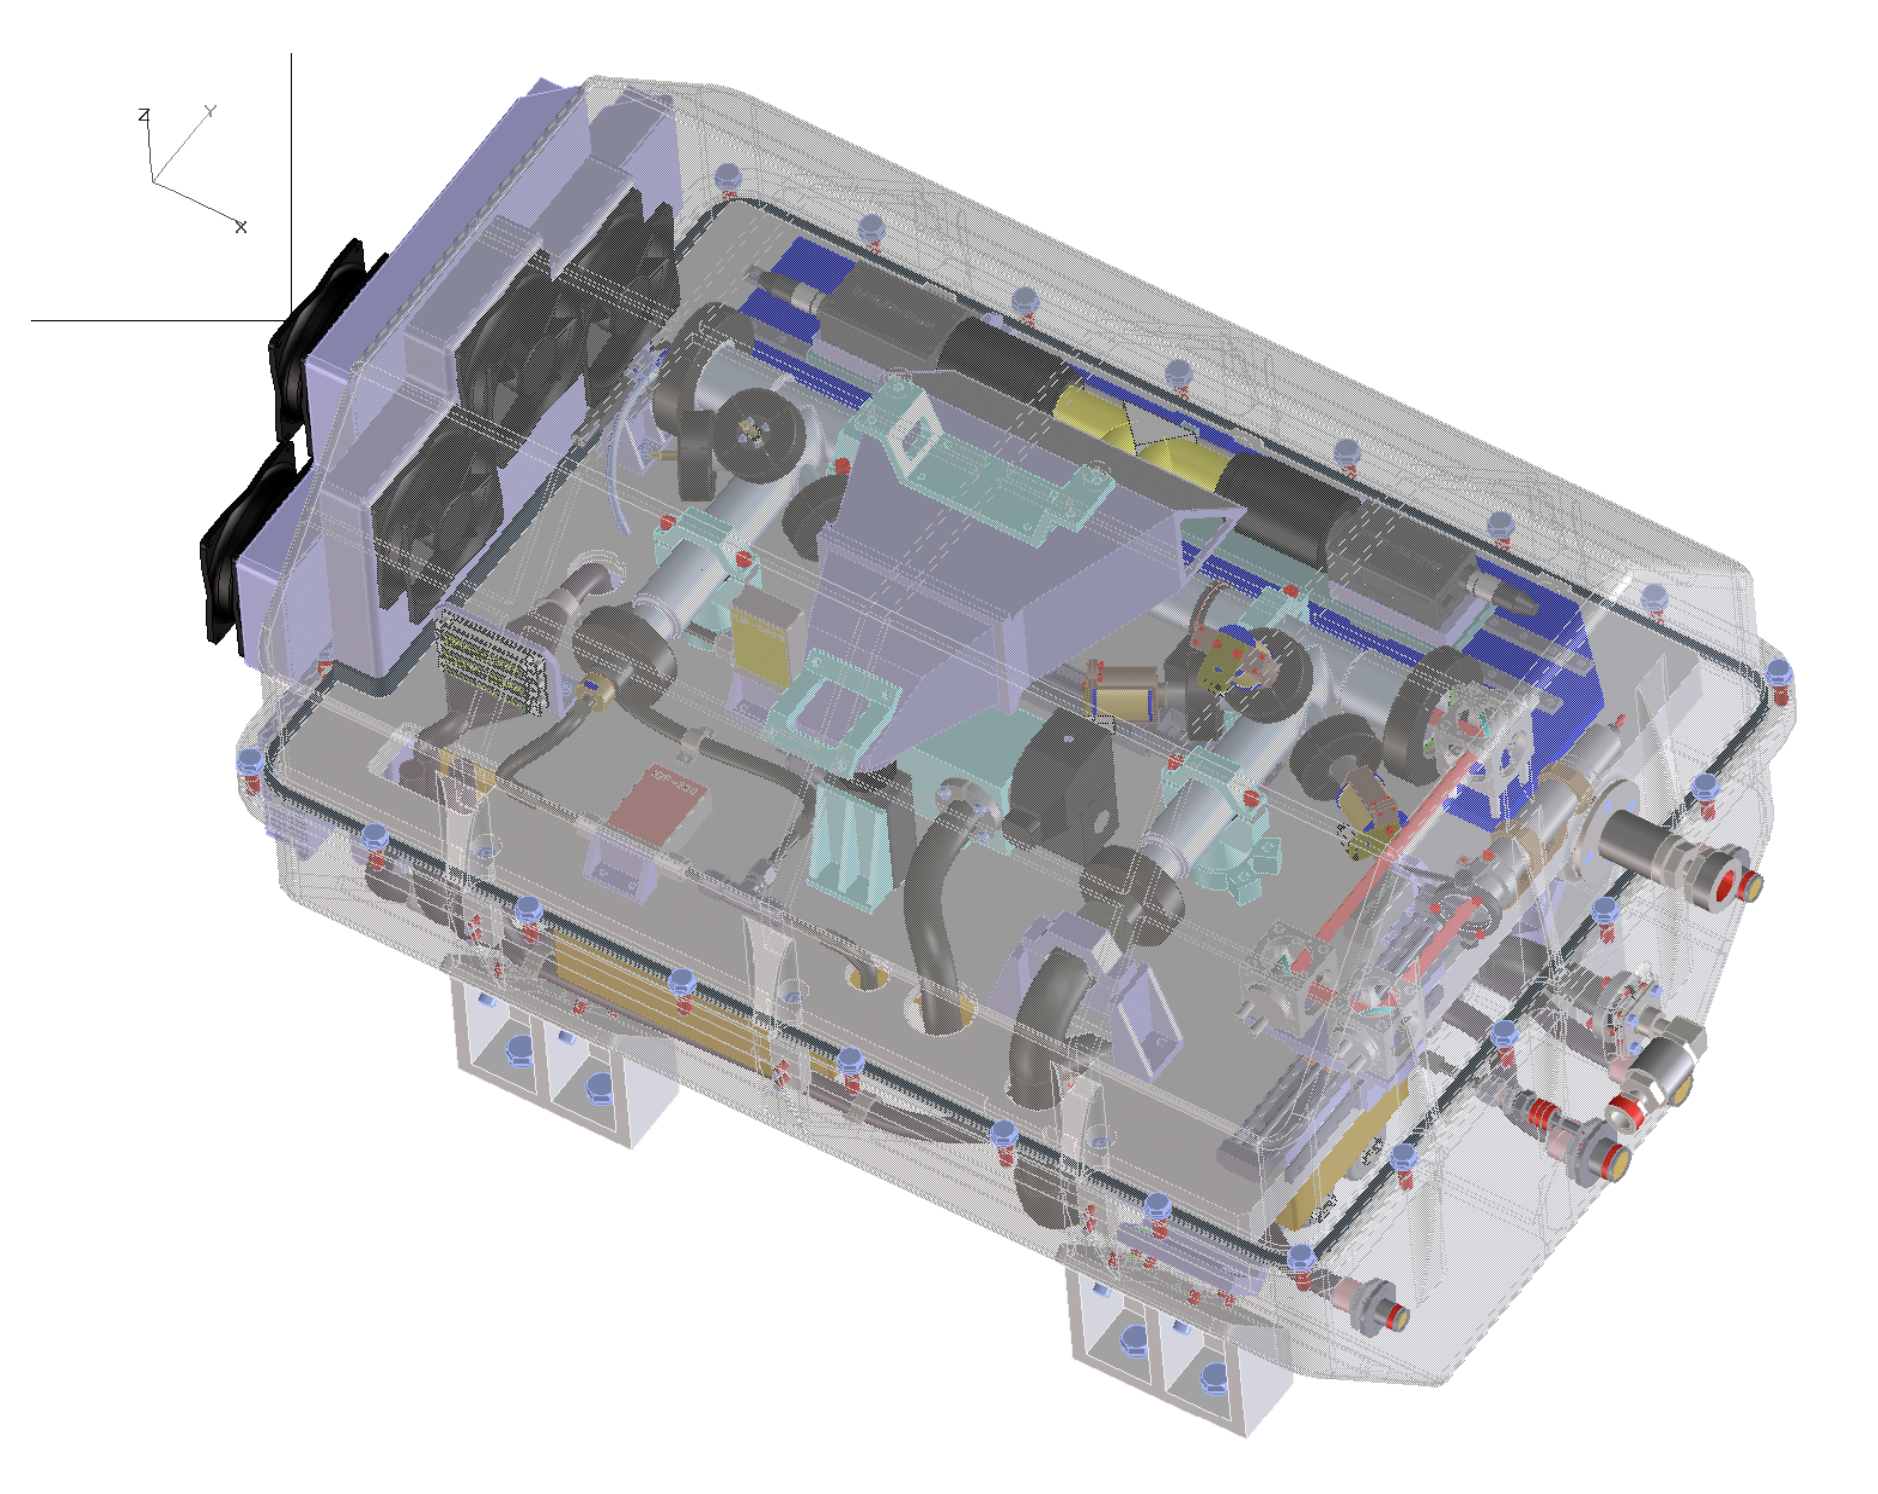
\includegraphics[width=0.35\textwidth]{figures/3D-scheme-pk4}
         }
         \hspace{0.05\columnwidth}
         \subfloat[\label{sub:photo-pk4}]{
           \includegraphics[width=0.35\textwidth]{figures/photo-pk4}
         }
         \caption{Экспериментальная установка космической аппаратуры “Плазменный~кристалл-4”: \pt(a) 3D-модель внутренностей,
                  \pt(b) фото уже собранной установки в лабораторных условиях.}
    \end{center}
    \label{fig:pk4}
\end{figure}

\section{Спектрометр “OceanOptics~USB2000+”}
Для осуществления спектральной диагностики КА~“ПК-4“ применяется модульный мини-спектрометр OceanOptics~USB2000+ (см~рис.~\ref{fig:usb2000+}).
В основе лежит 2048-пиксельная ПЗС-линейка, которая позволяет проводить спектральные измерения в диапазоне длин
волн 350-1100~нм со спектральным разрешением 1.5~нм. Приемная оптика спектрометра устанавливается рядом
с камерами высокого разрешения (CCD1, CCD2) и подключается к спектрометру через оптическое волокно (см~рис.~\ref{fig:fig31}).
Время считывания одного спектра составляет 4~с. Основная цель применения спектрометра в данной аппаратуре - это
контроль чистоты плазмы во время экспериментов на основе спектральных методов поиска примесей.
\begin{figure}[t]
  \centering
  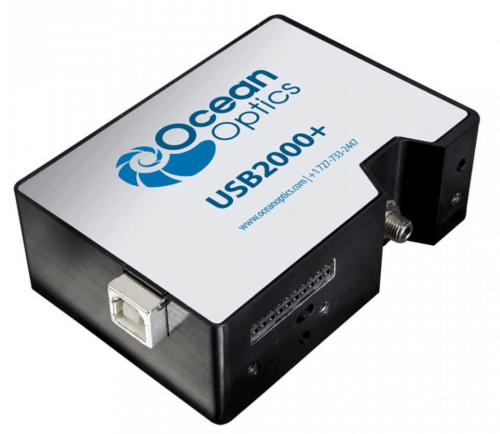
\includegraphics[width=12cm]{figures/usb2000+}
  \caption{Модульный мини-спектрометр OceanOptics~USB2000+.}
  \label{fig:usb2000+}
\end{figure}

\section{Экспериментальные данные}
\label{cha:ch_3_4}
В космической аппаратуре “Плазменный~кристалл-4” выделены следующие каналы получения экспериментальных данных,
которые были задействованы в какой-либо мере в данной работе:
\begin{enumerate}
    \item Видеозаписи с двух камер высокого разрешения CCD1 и CCD2 (см~рис.~\ref{fig:fig32}).
    Видеофайлы в сыром виде имеют формат “.avi” с размером 4~Gb/min от одной камеры. На данных записях хорошо
    различимы отдельные пылевые частицы, что позволяет отслеживать их траектории движения, а также наблюдать за
    их поведением в любой момент времени.

    \item Видеозаписи с общей камеры наблюдения. Представляют собой файлы в формате “.avi” с размером 0.3~Gb/min (см~рис.~\ref{fig:fig33}).
    На этих видеозаписях видно трубку целиком вместе с подсвеченной пылевой плазмой, где можно отследить макро поведение
    облака, в отличие от камер CCD1 и CCD2.

    \item Спектральные данные. Представляют собой текстовые файлы в формате “.dat”, которые имеют свою особую структуру
    по блокам, удобную для парсинга. Пример блока можно найти в \hyperref[app:app1]{приложении~А}. Эти спектральные данные
    хранят информацию о состоянии спектрометра в любой момент времени, его манипуляции, а также сырые данные с его ПЗС-линейки.

    \item Логи. Представляют собой текстовые файлы в формате “.log”, которые содержат информацию обо всех
    технических изменениях в ходе эксперимента с временными отметками. Пример также можно найти в \hyperref[app:app2]{приложении~Б}.
\end{enumerate}

\begin{figure}[t]
  \centering
  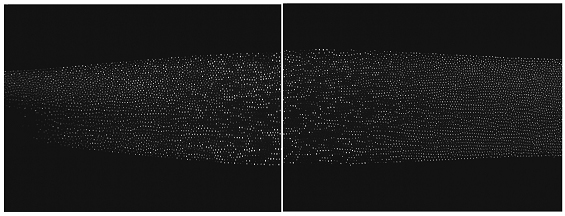
\includegraphics[width=12cm]{figures/fig32}
  \caption{Кадры видеозаписей с двух камер наблюдения высокого разрешения PGO. Кадры синхронизированы во времени, а также пространственно дополняют друг друга.}
  \label{fig:fig32}
\end{figure}

\begin{figure}[t]
  \centering
  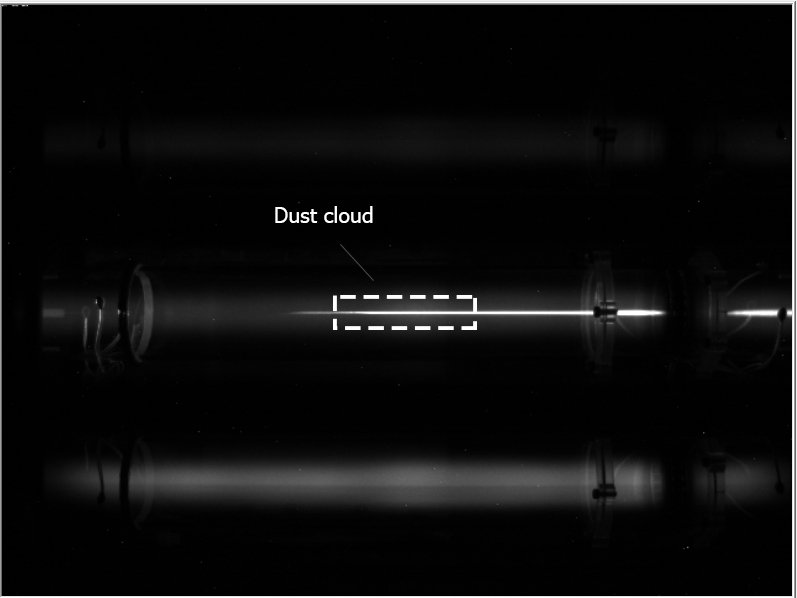
\includegraphics[width=6cm]{figures/fig33}
  \caption{Кадр видеозаписи с общей камеры наблюдения с отмеченным пылевым облаком.}
  \label{fig:fig33}
\end{figure}
\chapter{Программа “Spectral Analyzer PK-4”}
\label{cha:ch_4}
\section{Актуальность программы}
В ходе данной работы был создан веб-сервис “Spectral~Analyzer~PK-4”, название которого состоит из двух частей:
первая часть (“Spectral~Analyzer”) обозначает главную задачу сервиса - спектральный анализ, а вторая часть говорит
о том, что анализ осуществляется на данных, полученных с исследуемой в текущей работе экспериментальной установки
“Плазменный~кристалл-4” (PK-4). Какие задачи решает “Spectral~Analyzer~PK-4”?

Наиболее важная задача - это, собственно, обработка огромного количества спектральной информации, поступающей с борта МКС
Российско-европейской Космической Аппаратуры “Плазменный~кристалл-4”. Поскольку спектральные данные представляют собой
довольно сложную, но упорядоченную структуру данных (см раздел \ref{cha:ch_3_4}), то ручная обработка и
графическое построение даже одного спектра является времязатратной и трудоёмкой задачей: необходимо ориентироваться
в текстовых логах, а также владеть навыками работы, как минимум, с двумя программами одновременно~-~Origin и Exсel.
У умелого пользователя данных программ (при большом желании) получится построить один спектр не быстрее, чем за 5~мин.
Так как в одном эксперименте возможность встретить более 1000~спектров - обычное явление, то даже таких умений становится недостаточно.

Далее, ожидается, что веб-сервис даст инструмент первичной спектральной обработки: полиномиальная калибровка длин волн,
вычитание и усреднение шумового фона, автоопределение пиков спектральных линий, усреднение идентичных спектров при одних
и тех же параметрах и др.

Мотивационный момент, в будущем данный веб-сервис может быть полезен для подготовки датасетов для применения алгоритмов
машинного обучения.

Поскольку в данной работе разработана и применена методика поиска относительного изменения электронной температуры на основе
отношения интенсивностей спектральных линий, то для “Spectral~Analyzer~PK-4” ставится задача рассчета отношений интенсивностей
спектральных линий в зависимости от энергии верхнего уровня.

Еще один мотивационный момент, данный веб-сервис потенциально дает возможность взаимодействовать
с немецкими коллегами по космической аппаратуре ПК-4.

Таким образом, было решено создать автоматизированное компьютеризированное программное обеспечение для решения данных проблем.

\section{Требования к программе}
Чтобы было не только удобно и практично пользоваться и совершенствовать программу, но и для достижения решения
поставленных задач, были выдвинуты определенные требования к программе.

Во первых, программа должна обладать свойством кроссплатформенности, т.е. независимо от типа операционной
системы она должна работать корректно. Конкретнее, должна быть возможность работы под следующими операционными
системами: Windows~XP - Windows~10, MacOs, Linux с графической оболочкой.

Во вторых, программа должна иметь возможность сохранения ключевых состояний процесса обработки данных,
а также максимально безболезненно передавать прогресс между пользователями.

Далее, программа должна уметь в автоматическом режиме загружать и парсить текстовые спектральные данные
(эксперименты), а также отображать список уже загруженных экспериментов.

Следующий важнейший аспект - это умение динамически отображать более 1000~спектральных графиков в одном
рабочем окне, отображать метаинформацию по текущему спектру.

Для обработки спектров необходимо учитывать фоновое излучение, поэтому программа должна иметь возможность по
выбранным пользователем номерам спектров усреднять их интенсивности, а также вычитать из всех спектров текущего эксперимента.

Не менее важный аспект - это возможность настроить калибровку спектра по длине волны на основе вводимой пользователем полиномиальной функции.

Далее, для поиска отношений интенсивностей необходимо на основе откалиброванных незашумленных спектров сохранять
усредненные спектры-заготовки с учётом среднеквадратичных погрешностей, также необходимо отображать
список уже сохранённых усредненных спектров.

В силу того, что используемый спектрометр “OceanOptics~USB2000+” имеет невысокую разрешающую
способность (см раздел \ref{cha:ch_3_4}), то для корректного поиска отношений интенсивностей
необходимо учитывать наложения линий друг на друга с помощью аппаратной функции спектрометра,
т.е. следующее требование к программе: она должна уметь на основе полиномиального приближения аппаратной
функции учитывать перекрытия рядом стоящих линий с учетом погрешностей.

В данной работе особый интерес представляет зависимость отношения интенсивностей определенных линий от энергии
возбужденного состояния, для этого программа должна иметь библиотеку спектральных линий, а также функционал
по выбору набора линий при построении данной зависимости.

Таким образом, мы перечислили основные требования к программе, а сейчас разберем стек технологий,
который был изучен для достижения данных целей (см.~рис.~\ref{fig:it_tech}).
\begin{figure}[t]
  \centering
  
\includegraphics[width=12cm]{figures/it_tech}
  \caption{Изображены логотипы изученных IT-технологий, которые использовались для создания веб-сервиса “Spectral~Analyzer~PK-4”}
  \label{fig:it_tech}
\end{figure}

\section{Стек изученных технологий}
Первый прототип программы был написан традиционным образом на языке C\#, который непременно предполагает
стандартную установку под Windows и работу с программой, как с ПО для данной операционной системы.
В данном варианте было реализовано лишь около 20\% необходимого функционала, но при этом возникли большие трудности
с передачей программы научному руководителю из-за несовместимости версий Windows~7 и XP.

Для решения проблем кроссплатформенности и передачи данных между пользователями было решено создать веб-сервис,
который работает в обычном браузере, поскольку почти каждая операционная система с графической оболочкой
поддерживает большинство современных браузеров.

Django (Джанго)~--~свободный фреймворк для веб-приложений на языке Python, использующий шаблон проектирования MVC.
Проект поддерживается организацией Django Software Foundation \cite{Django}. Джанго имеет удобную гибкую
внутреннюю архитектуру, которая позволяет разработчикам, при достаточных знаниях, выполнять огромный спектр задач
из области веб-программирования. Перечислять все возможности данного фреймворка нет необходимости, подчеркнем лишь те,
что были использованы для решения поставленных задач.

Джанго имеет свою стандартизированную ORM, которая поддерживает транзакции. ORM (англ. Object-Relational Mapping,
рус. объектно-реляционное отображение или преобразование)~--~это некая оболочка над базой данных, которая позволяет
использовать функционал базы данных с помощью объектно-ориентированного языка программирования, в данном случае с помощью Python.

Далее, в Джанго есть система маршрутизации урлов, которая позволяет настраивать POST и GET запросы на основе регулярных выражений,
что очень удобно: в Python есть хорошо известный и понятный встроенный модуль “re”, который почти ничем не отличается по синтаксису.

В Джанго предусмотрена возможность применения криптографически шифрованных Cookie и CSRF-токенов для защиты POST
запросов к серверу: например, для аутентификации пользователя, для любого изменения и некоторых запросов к информации сервера.
Это дает довольно хорошую защиту от мошеннических и хакерских атак.

PostgreSQL~--~свободная объектно-реляционная система управления базами данных, разработанная в Калифорнийском
университете на факультете компьютерных наук в Беркли \cite{PostgreSQL}. PostgreSQL поддерживает большой набор встроенных типов данных:
\begin{itemize}
\item численные типы;
\item двоичные типы;
\item типы «дата/время»;
\item булев тип;
\item перечисление;
\item геометрические примитивы;
\item UUID-идентификатор;
\item XML-данные;
\item массивы;
\item JSON;
\item идентификаторы объектов БД;
\item псевдотипы;
\end{itemize}

NumPy является основным пакетом для научных вычислений в Python, которая поддерживает
многомерные массивы (в~т.ч.~матрицы), а также предоставляет прекрасно оптимизированные высокоуровневые методы для работы с ними,
включая математические, логические, манипуляции с размерностью, сортировку, отбор, ввод-вывод, дискретные преобразования Фурье,
основную линейную алгебру, основные статистические операции, случайное моделирование и многое другое \cite{Numpy}.
Исходный код NumPy находится в открытом доступе.

SciPy — библиотека для языка программирования Python с открытым исходным кодом, предназначенная для выполнения научных и
инженерных расчётов \cite{Scipy}. Возможности:
\begin{itemize}
\item поиск минимумов и максимумов функций;
\item вычисление интегралов функций;
\item поддержка специальных функций;
\item обработка сигналов;
\item обработка изображений;
\item работа с генетическими алгоритмами;
\item решение обыкновенных дифференциальных уравнений;
\end{itemize}

CanvasJS - библиотека для языка программирования JavaScript, которая предоставляет API для работы с диаграммами и графиками
в веб-проектах. Для студентов и некоммерческого использования лицензия предоставляется бесплатно. Основные преимущества:
\begin{itemize}
\item простой API;
\item высокая производительность;
\item 30 типов диаграмм;
\item хорошая документация;
\item поддержка браузеров Chrome, Firefox, Safari, IE8+;
\end{itemize}

При создании веб-сервиса “Spectral~Analyzer~PK-4“ использовались следующие версии библиотек:
\begin{itemize}
\item django==2.0;
\item psycopg2==2.7.1;
\item numpy==1.14.2;
\item django-debug-toolbar==1.8;
\item scipy==1.0.1;
\item python-dateutil==2.6.1;
\item canvas-js==2.1
\end{itemize}

\section{Описание функционала}
Используя описанный стек технологий был создан веб-сервис “Spectral~Analyzer~PK-4” версии 1.0.0.
В данном разделе находится информация о том, как пользователь взаимодействует с сервисом данной версии, описание функционала
и некоторые решения на программном уровне, которые показались автору интересными/полезными для прочтения.

С точки зрения установки данного программного обеспечения все сильно упрощено~--~достаточно лишь открыть URI
сервиса в своем браузере и начать работу. Таким образом пользователь освобождается от трудоемких операций по получению ПО
и может пользоваться сервисом с любой точки мира, почти с любого устройства, имеющего совместимую версию браузера.

Первое взаимодействие с пользователем начинается со страницы аутентификации (см.~рис.~\ref{sub:auth}). На данном
этапе проходит проверка пользователя на наличие доступа к контенту: необходимо ввести почту и пароль, выданные разработчиками
сервиса. На программном уровне пользователь имеет следующую ORM абстракцию:

\begin{figure}[t]
    \begin{center}
         \subfloat[\label{sub:auth}]{
           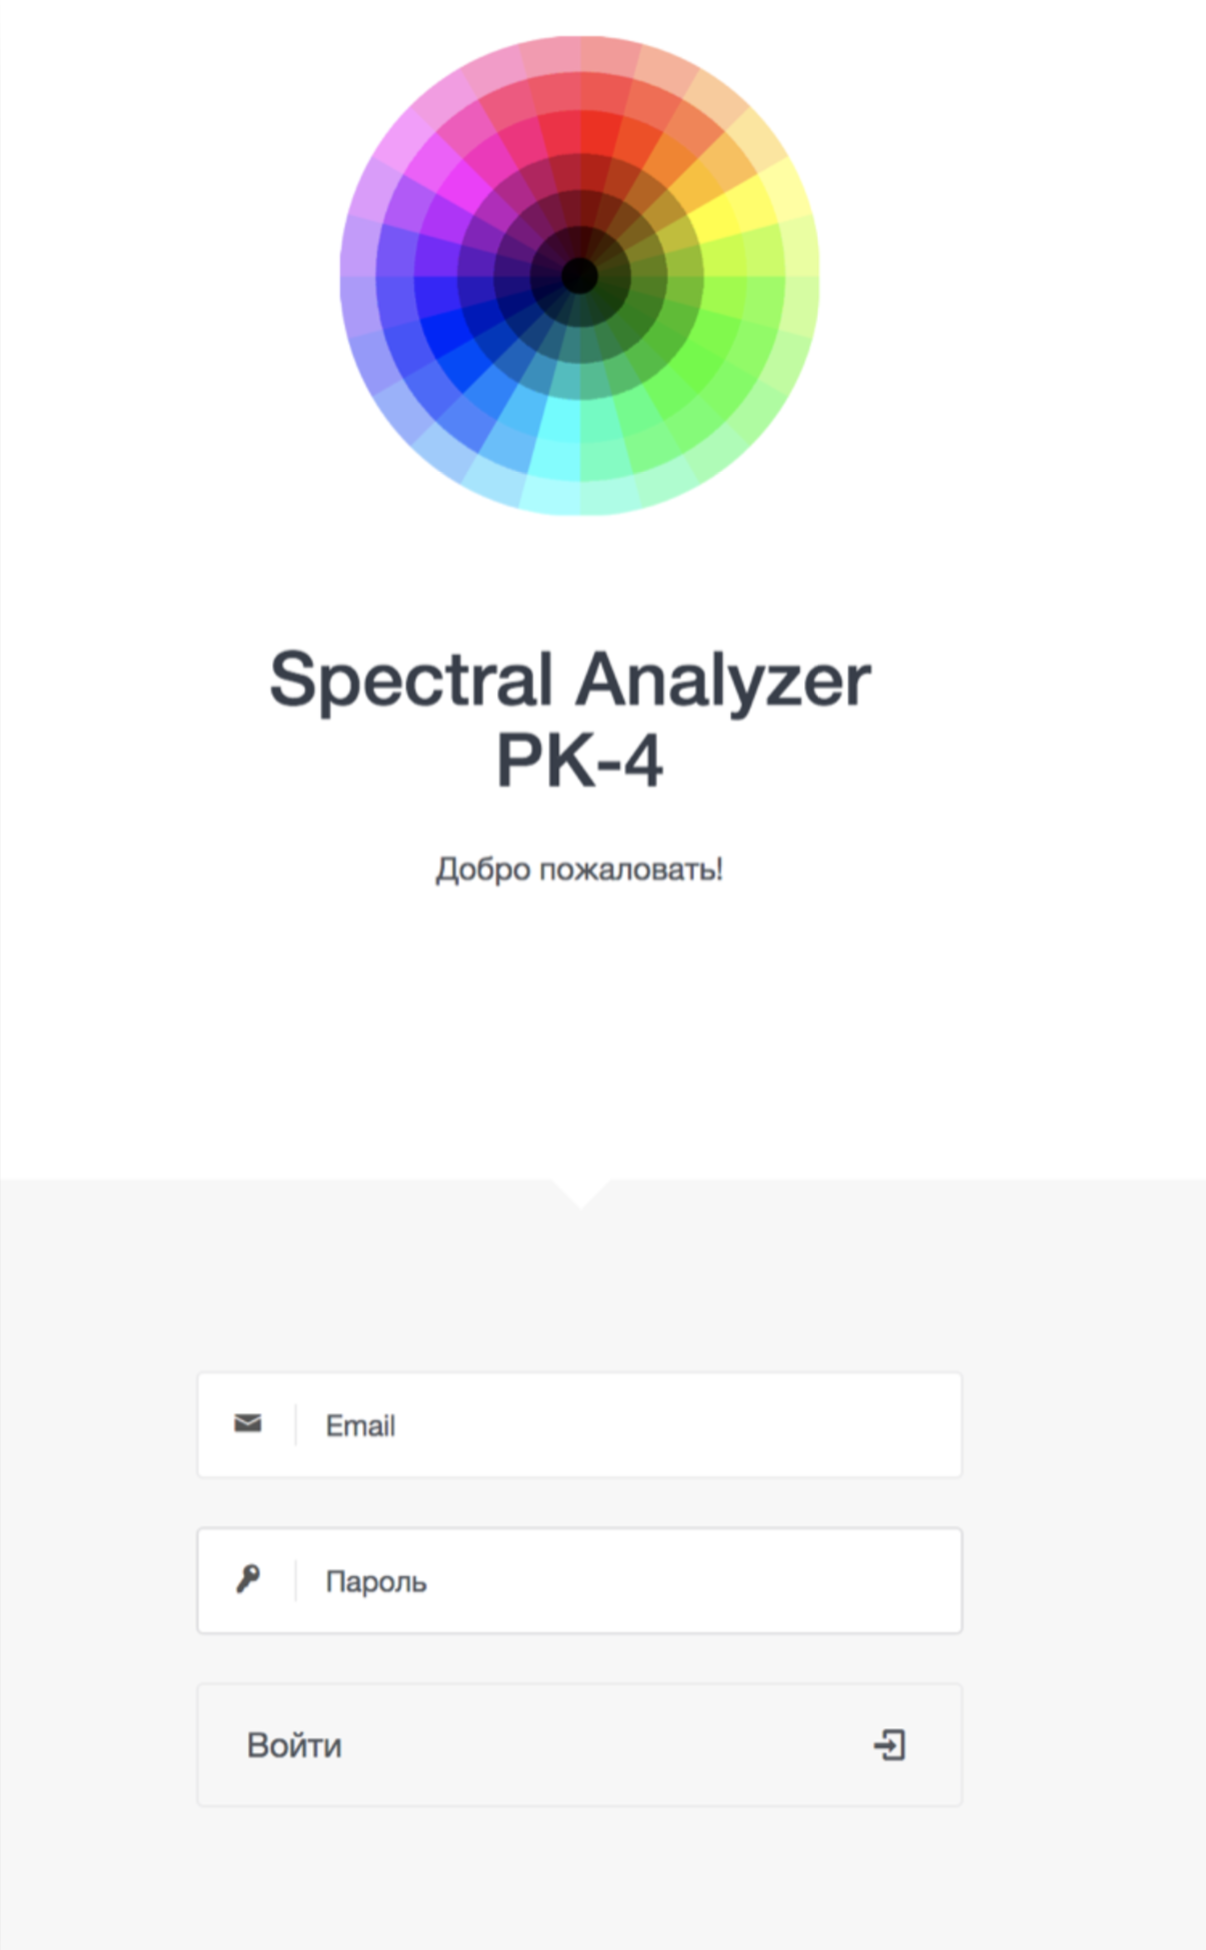
\includegraphics[width=0.35\textwidth]{figures/auth}
         }
         \hspace{0.05\columnwidth}
         \subfloat[\label{sub:page_not_found}]{
           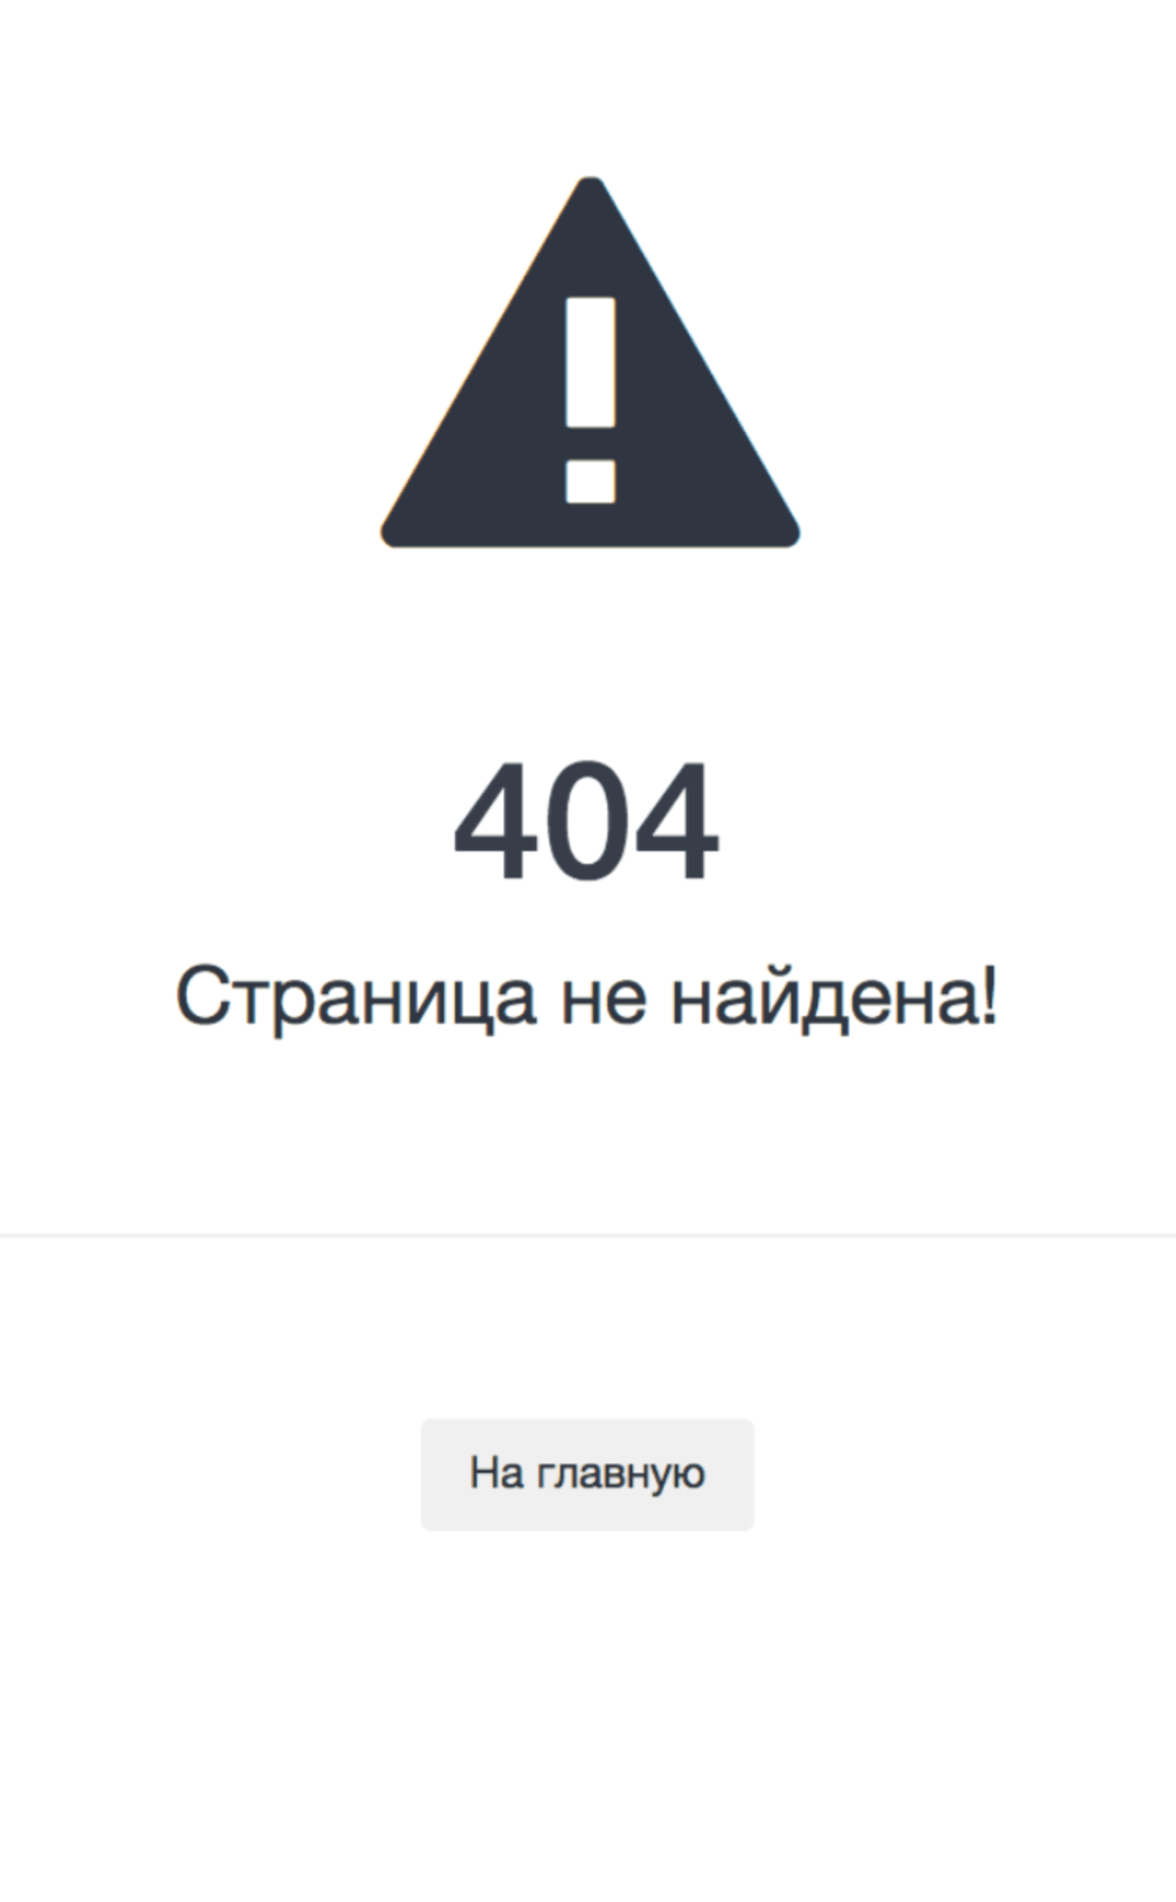
\includegraphics[width=0.35\textwidth]{figures/page_not_found}
         }
         \caption{Страницы в веб-сервисе “Spectral~Analyzer~PK-4”.: \pt(a) аутентификации, \pt(b) отсутствие страницы.}
         \label{fig:auth_and_page_not_found}
    \end{center}
\end{figure}

\begin{lstlisting}[style=py]
from django.contrib.auth.base_user import AbstractBaseUser
from django.contrib.auth.models import UserManager
from django.db import models

class User(AbstractBaseUser):
    email = models.EmailField(unique=True)
    first_name = models.CharField(max_length=64)
    last_name = models.CharField(max_length=64)
    institute = models.ForeignKey(Institute, models.DO_NOTHING)
    objects = UserManager()
    USERNAME_FIELD = "email"
\end{lstlisting}
У пользователя есть уникальная почта в системе, имя и фамилия, определена принадлежность к институту,
а также базовые параметры: хешированный пароль и время последней аутентификации.

На примере аутентификации разберем как происходят POST и GET запросы к удаленному веб-сервису, поскольку технически
данный подход ничем не отличается от получения информации по спектрам. Запрос GET используется для получения
содержимого указанного ресурса. С помощью метода GET можно также начать какой-либо процесс. Клиент может передавать
параметры выполнения запроса в URI целевого ресурса после символа «?»:
\begin{verbatim}
GET /login?param1=value1&param2=value2 HTTP/1.1
\end{verbatim}
Таким образом браузер выступает в роли клиента и выполняет GET запрос на удаленный сервер, который уже понимает специфику
HTTP протокола и предпринимает соответствующее действие. На примере аутентификации, при выполнении GET запроса должна
отобразиться страница, где, собственно, можно пройти аутентификацию (см.~рис.~\ref{sub:auth}). Для выполнения ответа
на данный запрос веб-сервис сверяет URL в соответствии со списком "urlpatterns":
\begin{lstlisting}[style=py]
from django.conf.urls import url
from web.views import LoginView

urlpatterns = [url(r"^login$", LoginView.as_view())]
\end{lstlisting}
Если не нашлось совпадения URL по регулярному выражению, то отоборажается ошибка 404 “Not Found” (см.~рис.~\ref{sub:page_not_found}),
а в случае совпадения выполняется действие, которое задается методом “get” класса LoginView:
\begin{lstlisting}[style=py]
from django.views.generic import View
from django.http import JsonResponse
from django.conf import settings
from django.shortcuts import render, redirect
from django.contrib.auth import authenticate, login, REDIRECT_FIELD_NAME

from web.models import User

class LoginView(View):

    def get(self, request):
        if request.user.is_authenticated:
            return redirect("/base")
        return render(request, "web/login.html")

    def post(self, request, redirect_field_name=REDIRECT_FIELD_NAME):
        def error(error_text):
            return JsonResponse({"error": error_text}, status=401)

        redirect_to = request.POST.get(redirect_field_name, settings.LOGIN_REDIRECT_URL)
        # Ensure the user-originating redirection url is safe.
        if not is_safe_url(url=redirect_to, host=request.get_host()):
            redirect_to = settings.LOGIN_REDIRECT_URL

        if "email" not in request.POST:
            return error("Email required")
        if "password" not in request.POST:
            return error("Password required")

        email = request.POST["email"].strip().lower()
        password = request.POST["password"]
        try:
            User.objects.get(email=email)
        except User.DoesNotExist:
            return error("Invalid email")

        user = authenticate(email=email, password=password)
        if user is None:
            return error("Invalid password")

        login(request, user)
        return JsonResponse({"redirect_url": redirect_to})
\end{lstlisting}
В методе “get” содержится логика, что если пользователь прошел аутентификацию, то не нужно требовать проходить ее еще раз,
а необходимо перенаправить на основную страницу. В случае если аутентификация не пройдена, то необходимо отобразить
html-страницу “web/login.html”.

В случае с POST запросами все немного сложнее. Они применяются для передачи пользовательских данных заданному ресурсу.
Логика с определением “команды для сервера” остается такой же, как и в GET запросе, но сам запрос отличается своей структурой:
данные необходимо передавать в тело запроса. Поскольку передача пользовательских данных требует безопасности, то
необходима защита. Например, в Джанго можно выставить требование на передачу CSRF-токена для любого POST-запроса.
Что это значит? CSRF-токен является последовательностью символов, которая передается вместе с ответом на GET запрос,
причем на каждый ответ сервер генерит новую последовательность, отличную от предыдущей. Если в POST запросе не был прислан
CSRF-токен или присланный токен не совпадает со сгенерированным сервером, то сервер отклоняется действие. Таким образом, можно
избежать межсайтовой подделки запроса и быть уверенными, что это реальный пользователь, а не злоумышленник.
На стороне клиента для совершения POST запросов в данном веб-сервисе используются
классические формы, после заполнения которых происходит POST-запрос, а также JQuery Ajax, если нет необходимости
перезагружать страницу для обновления данных:
\begin{figure}[t]
  \centering
  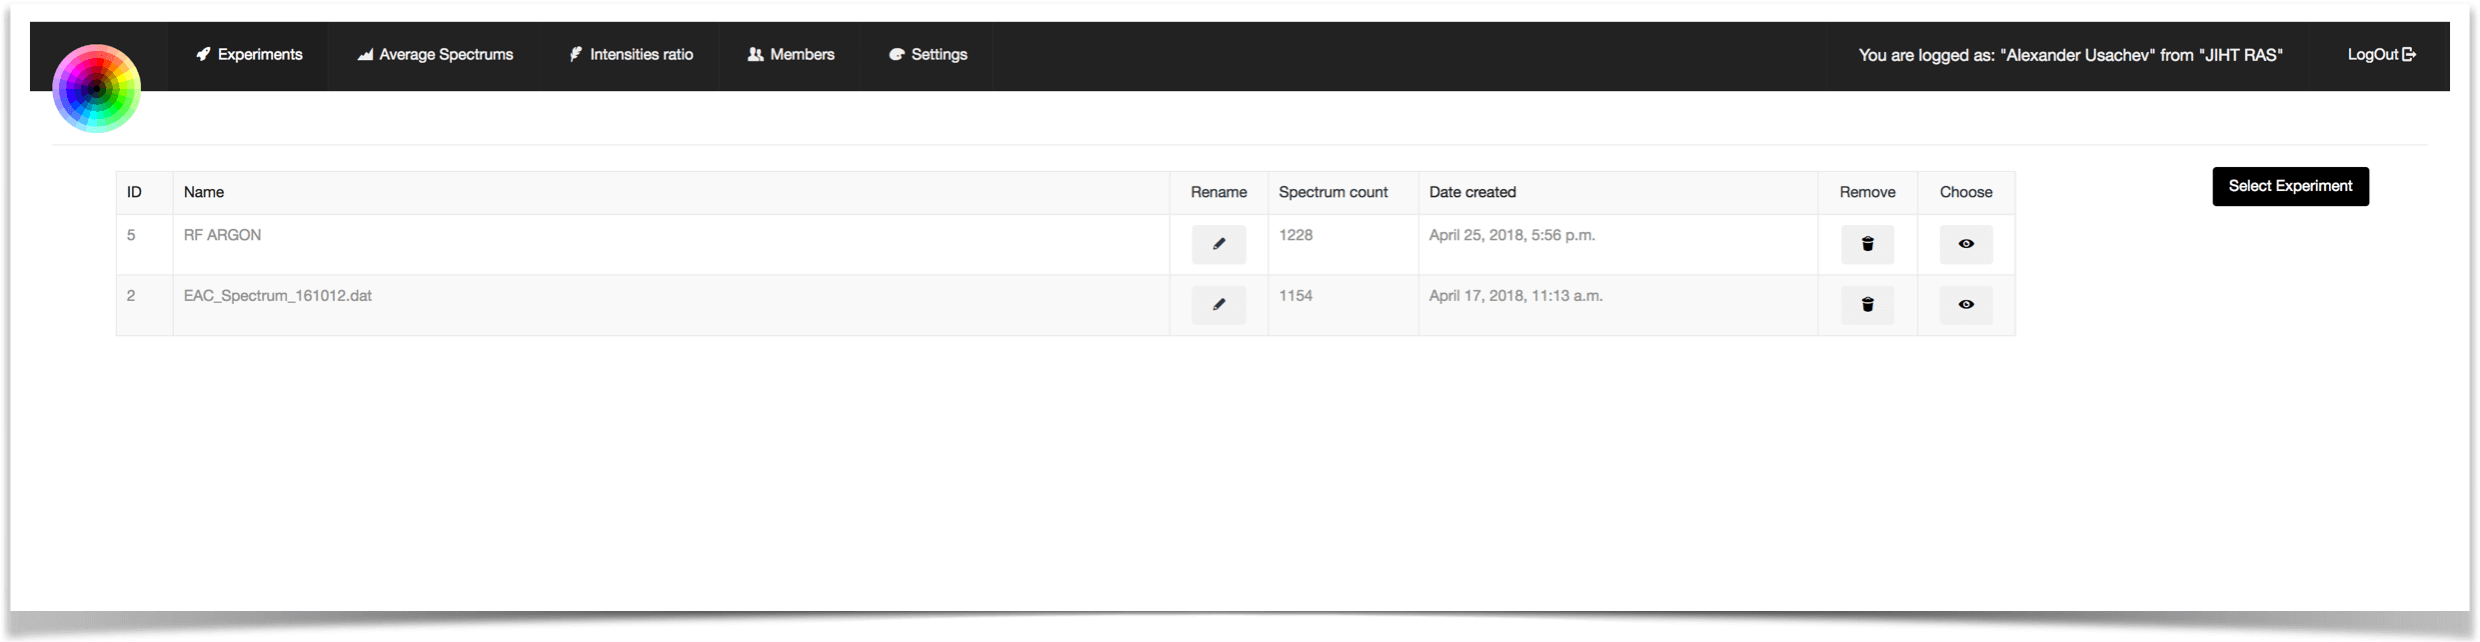
\includegraphics[width=16cm]{figures/all_experiments}
  \caption{Изображен результат рендеринга страницы “/all\_experiments” веб-сервиса “Spectral~Analyzer~PK-4”.}
  \label{fig:all_experiments}
\end{figure}
\begin{lstlisting}[style=htmlcssjs]
// Send data to the server
$.ajax({
    url: "/login",
    method: "POST",
    data: {
        email: $("input#email").val(),
        password: $("input#password").val(),
        next: $("input[name=next]").val(),
        csrfmiddlewaretoken: $("input[name=csrfmiddlewaretoken]").val(),
    },
    error: function(response) {
        <some_action>
    },
    success: function(response) {
        <some_action>
    }
});
\end{lstlisting}
Выполняя данный запрос, веб-сервис реагирует методом “post” класса “LoginView”, в котором содержится логика, что
если почта или пароль отстутсвуют, или, если нет пользователя с данной почтой, или пароль не совпадает, то аутентификация не пройдена
и надо это сообщить пользователю, а иначе перенаправить на основную страницу веб-сервиса.

Примерно на таком уровне проходит взаимодействие между пользователем и сервисом на программном уровне.
Необходимо придерживаться данных правил и задавать свои действия для методов “get” и “post” в соответствующем
наследнике класса “View”.


Итак, выполнив аутентификацию, пользователь попадает на основную страницу “Spectral~Analyzer~PK-4” с URL “/all\_experiments”
(см.~рис.~\ref{fig:all_experiments}), которая содержит:
\begin{itemize}
\item общее для всех меню, необходимое для навигации по сервису, в котором также содержится кнопка для выхода из системы,
а также имя, фамилия и институт авторизованного пользователя;
\item таблицу с уже загруженными экспериментами, в которой отображены ID, название, дата загрузки и количество спектров
в эксперименте. Также в таблице есть кнопки для переименования, удаления и просмотра эксперимента;
\item кнопку для загрузки и парсинга сырого файла со спектрами в формате “.dat”, данная процедура проводит запись в базу
данных;
\end{itemize}


\chapter{Анализ спектральных данных}
\label{cha:ch_5}

Данная глава посвящена анализу экспериментальных данных, в результате которого планируется
получить подтверждение или опровержение согласования теоретических расчетов (см.~раздел~\ref{sec:link_ratio_and_TE})
с экспериментом, оценить осевое электрическое поле $E_z$ и электронную температуру $T_e$ для электронов, участвующих
в неупругих столкновениях, в возмущенном пылевыми частицами положительном столбе газового разряда
постоянного тока.
\section{Лабораторный журнал}

Как и было описано в разделе~\ref{sec:experiment} на борту МКС на научной аппаратуре «Плазменный~кристалл~-~4»
был проведен нужный космический эксперимент 4 июня 2015 года с 16:04:26 до 16:05:38. В результате которого были
получены видеофайлы «VM1-AVI-150604-160426.avi» (левая камера высокого разрешения CCD1),
«VM2-AVI-150604-160427.avi» (правая камера высокого разрешения CCD2), «VM3-AVI-150604-160428.avi» (общая камера наблюдения CCD3),
файл со спектральными данными «EAC\_Spectrum.dat», а также файл с логированием всех действий «PK4-particletrappingmanipulation.log».
Спектральные данные для первого спектра в эксперименте представлены в \hyperref[app:app1]{приложении А},
а логи за все время эксперимента приведены в \hyperref[app:app2]{приложении~Б}.

В ходе сопоставления полученных данных действительности и синхронизации всех каналов между собой, были сделаны
следующие лабораторные записи:

\begin{figure}[t]
    \centering
    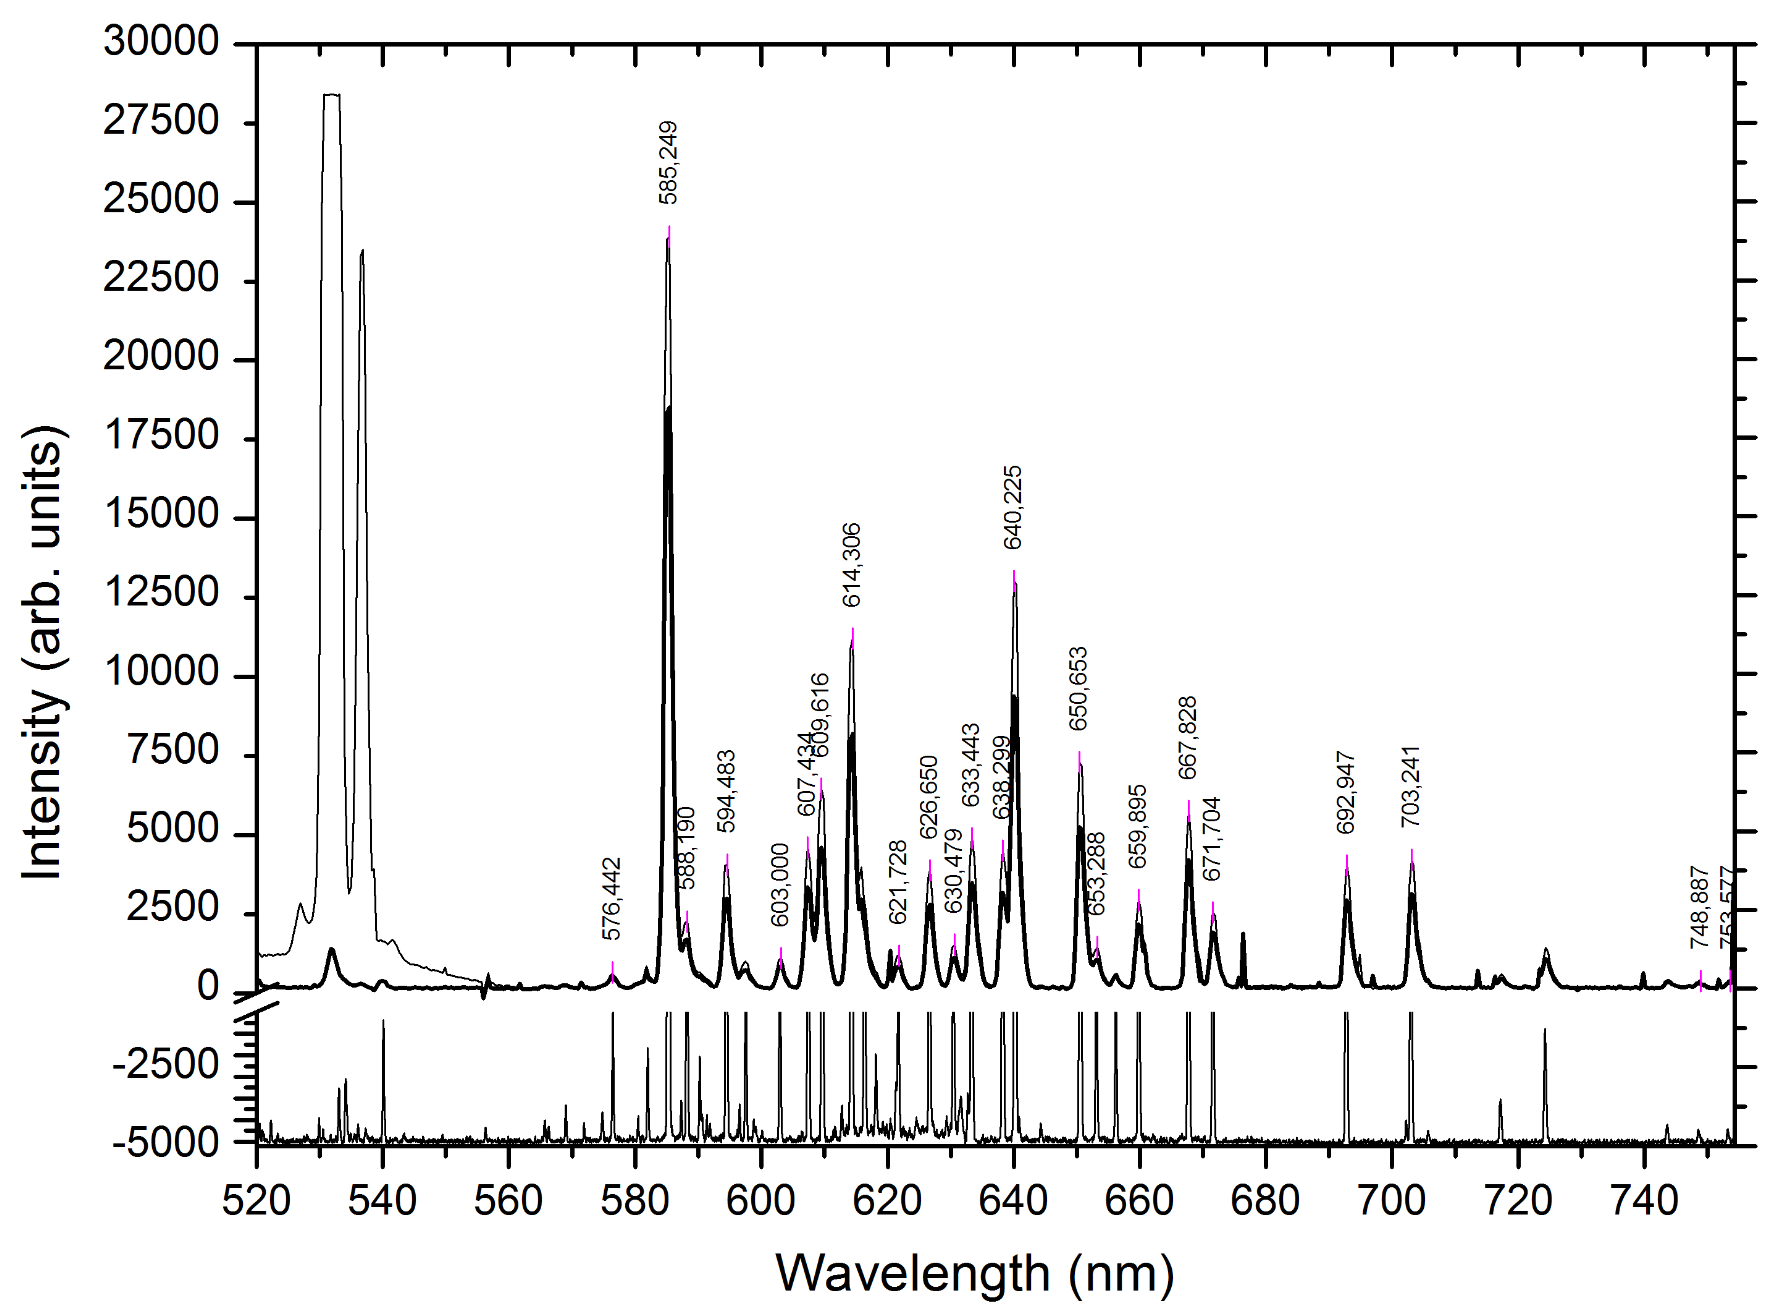
\includegraphics[width=16cm]{figures/main_spectrum}
    \caption{
        Наложенные спектры для трех конфигураций, усредненные и откалиброванные по длинам волн:
        жирной линией выделен спектр без пылевого облака; тонкой линией выделен спектр с пылевым облаком;
        ниже нуля достоверный спектр высокого разрешения атомарного неона.
    }
    \label{fig:main_spectrum}
\end{figure}

\begin{enumerate}
    \item Видео с левой камеры высокого разрешения CCD1:
    \begin{enumerate}
        \item отсутствие облака, время на видео: 0~--~33~с и 58~--~72~с;
        \item хорошая видимость облака, время на видео: 36~--~46~с;
    \end{enumerate}
    \item Видео с правой камеры высокого разрешения CCD2:
    \begin{enumerate}
        \item отсутствие облака, время на видео: 0~--~31~с и 59~--~71~с;
        \item хорошая видимость облака, время на видео: 35~--~53~с;
    \end{enumerate}
    \item Спектральные данные:
    \begin{enumerate}
        \item темновой ток, номера спектров: 52~--~55
        \item отсутствие облака, номера спектров: 888~--~895 и 903~--~904;
        \item хорошая видимость облака, номера спектров: 897~--~900;
    \end{enumerate}
    \item логи экспериментов не противоречат философии эксперимента: параметры разряда искусственно не менялись;
\end{enumerate}

\begin{figure}[t]
    \centering
    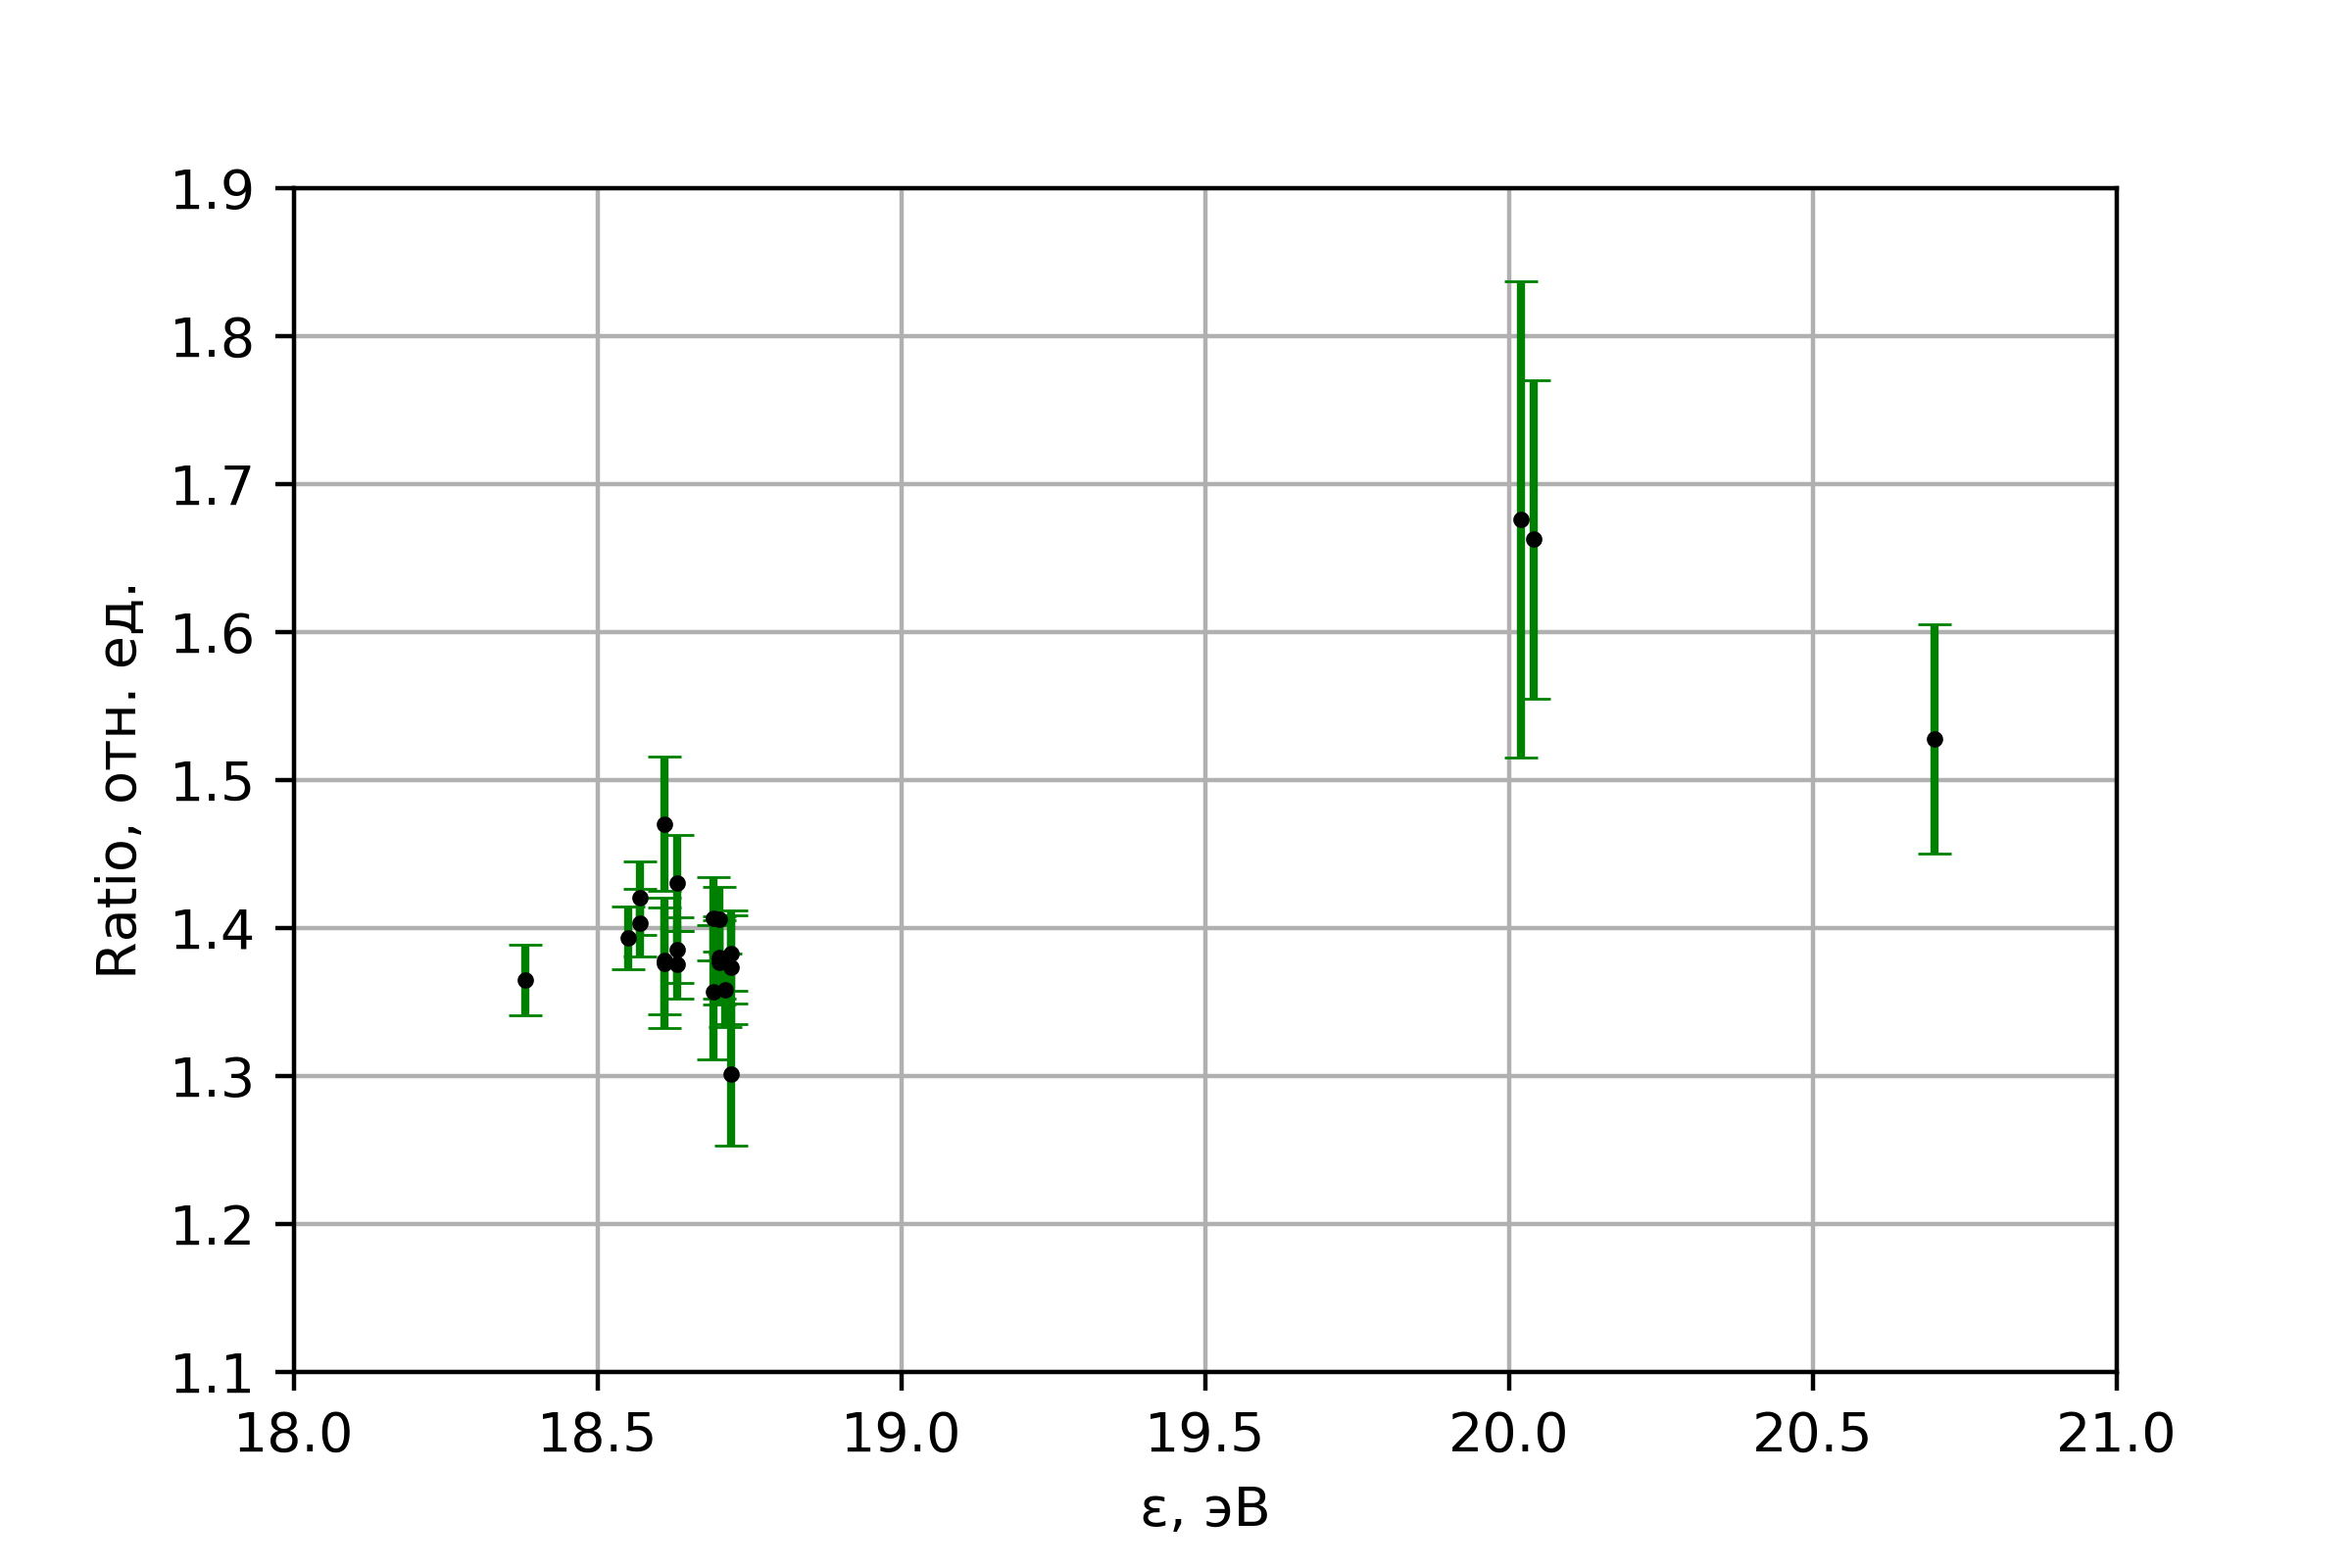
\includegraphics[width=16cm]{figures/experimental_ratio}
    \caption{Зависимость отношения интенсивностей спектральных линий неона в присутствии пылевого облака к отсутствию пылевого облака, полученного экспериментальным путем.}
    \label{fig:experimental_ratio}
\end{figure}

\section{Первичная обработка спектральных данных, наблюдение эффекта}

Для первичной обработки спектров, а именно для вычитания шумов и усреднения идеологически одинаковых спектров,
предлагается воспользоваться программой «Spectral~Analyzer~PK4», которая умеет обрабатывать спектры с НА~ПК-4 с учетом
среднеквадратичных погрешностей. Далее, были идентифицированы по длинам волн спектральные линии атомарного неона с помощью справочника
[?..ссылка~на~справочник..?] и спектра неона, полученного с помощью спектрометра высокого разрешения [?..ссылка~на~источник..?].
Для наглядности были наложены на один график
спектр невозмущенного состояния положительного столба газового разряда постоянного тока,
спектр возмущенного пылевым облаком положительного столба газового разряда постоянного тока и
спектр высокого разрешения для атомарных линий неона, а также отмечены идентифицированные линии~(см.~рисунок~\ref{fig:main_spectrum}).
Из данного рисунка следует отметить, что экспериментально наблюдается увеличение интенсивностей спектральных
линий при попадании пылевого облака в положительный столб газового разряда постоянного тока,
а также появление 532~нм сильного излучения, которое получено за счет рассеяния на пылевых частицах
532~нм лазерного ножа, используемого для подсветки.
\begin{figure}[t]
  \centering
  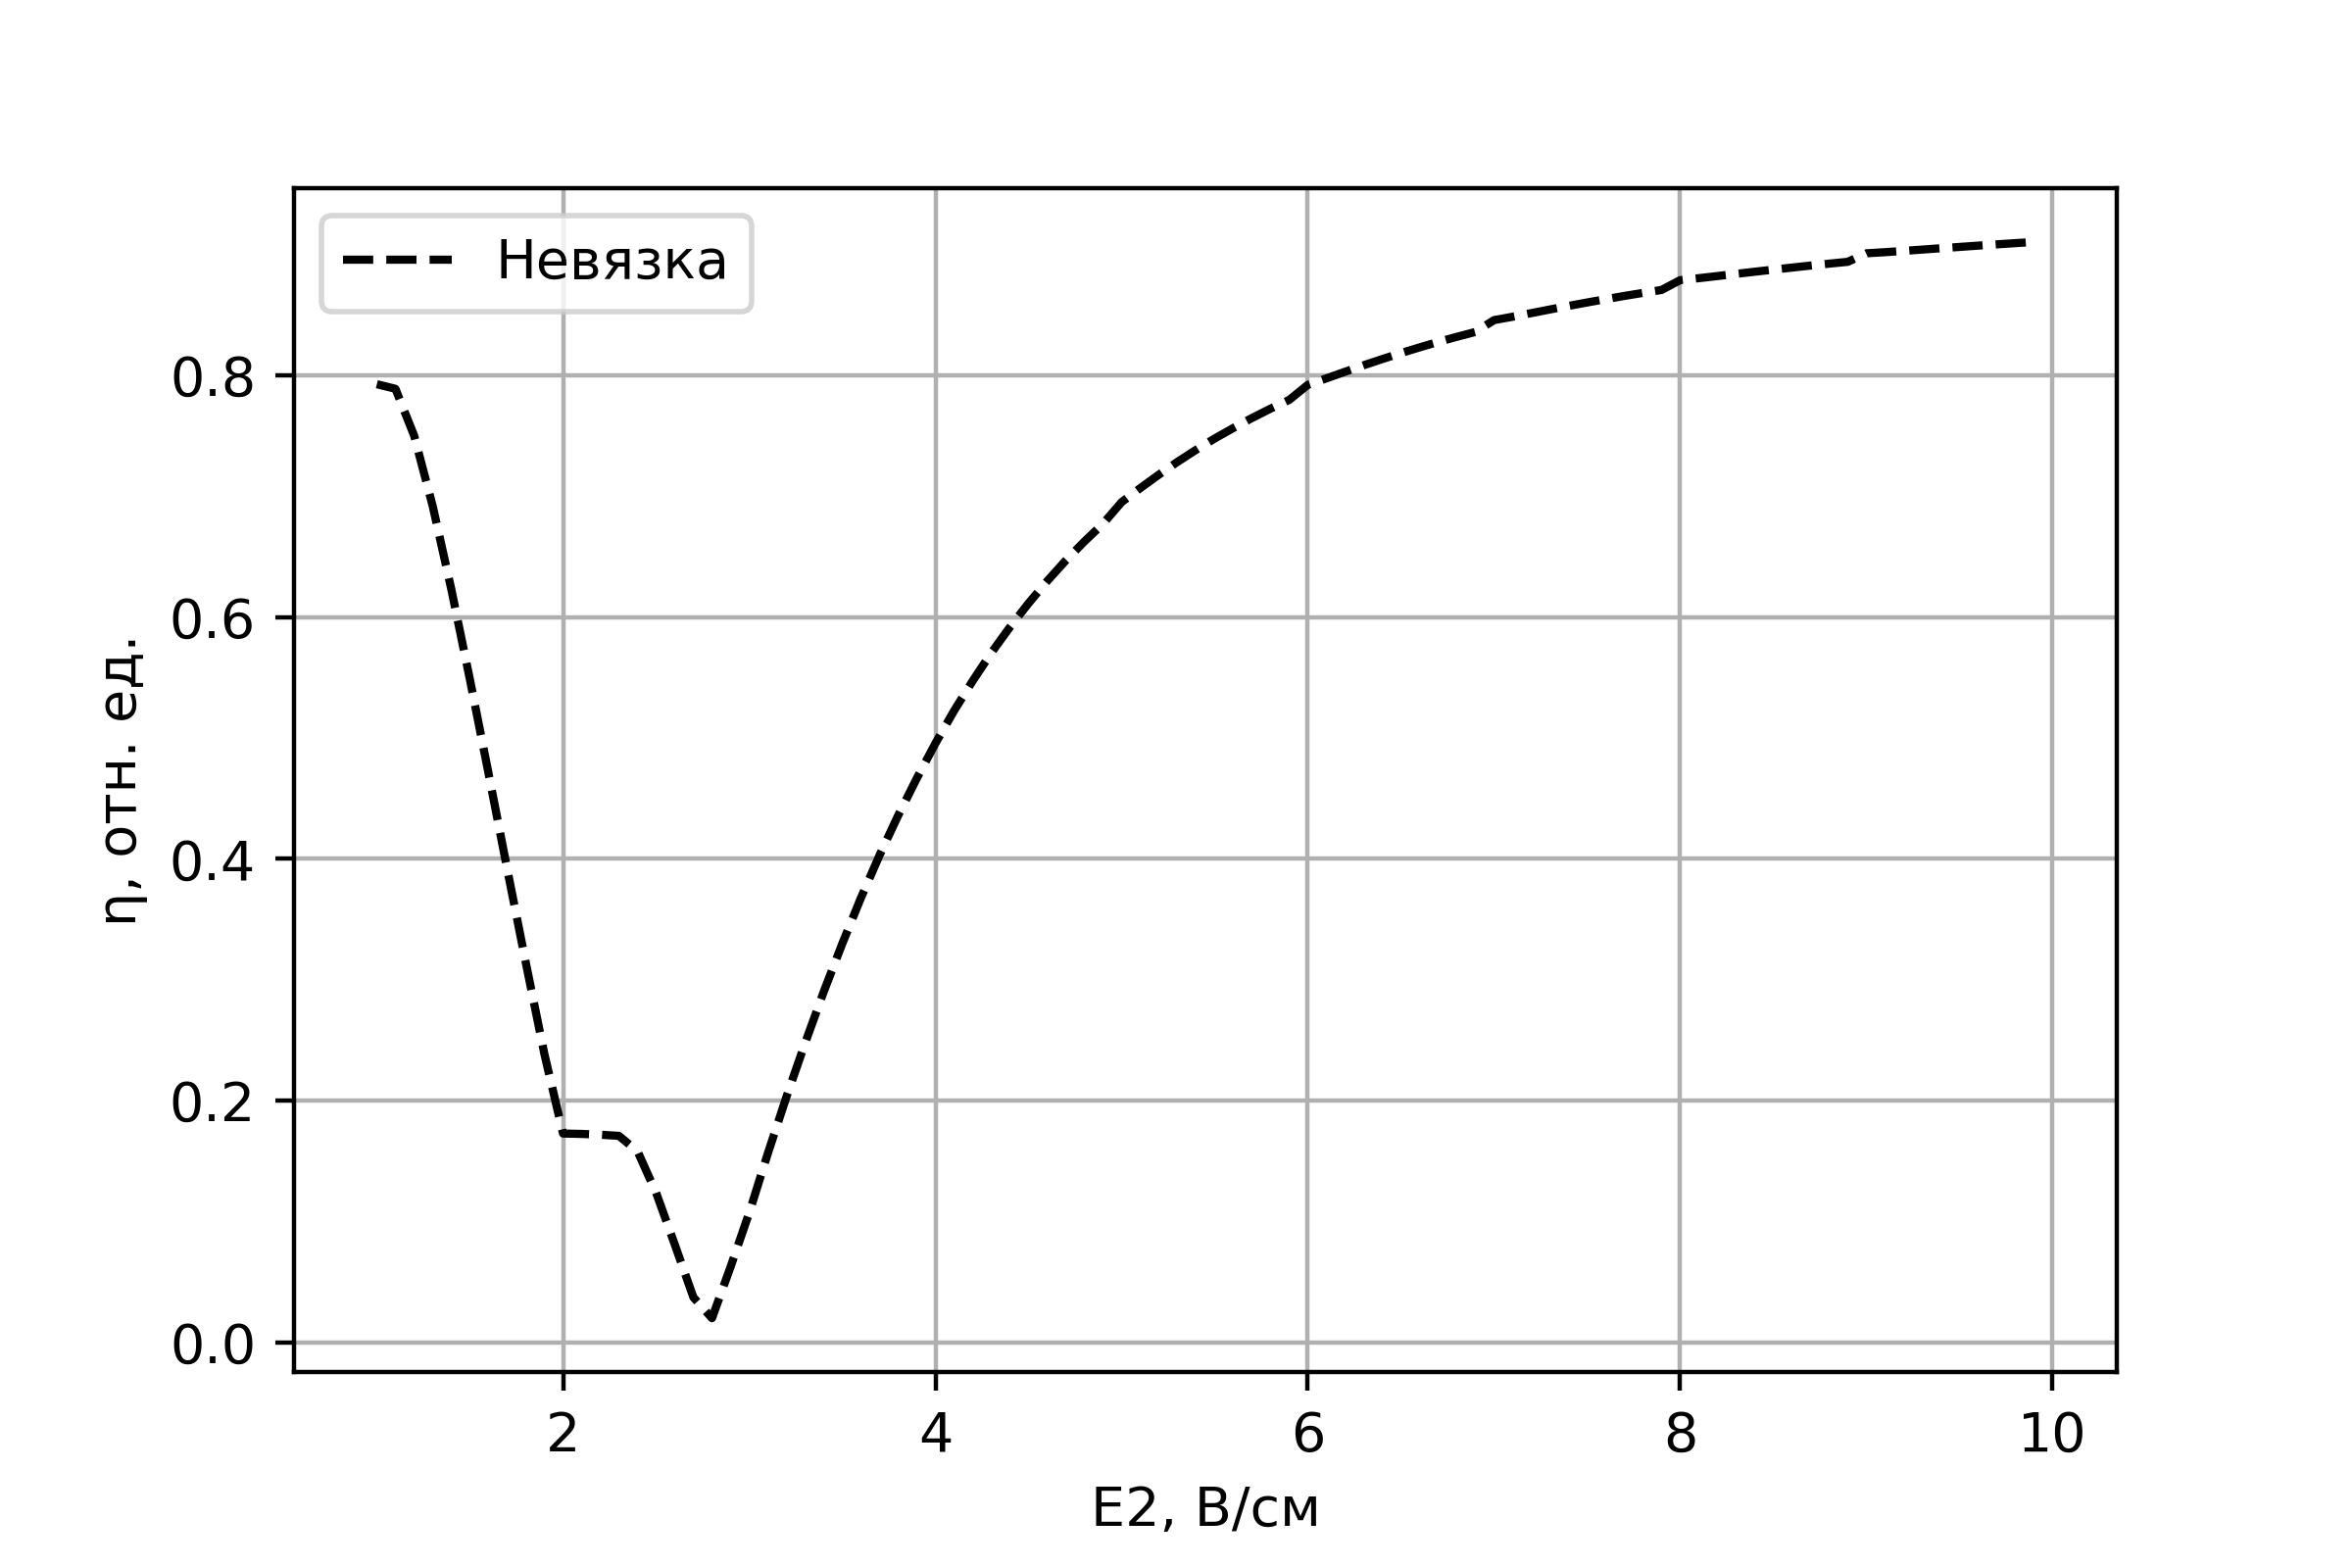
\includegraphics[width=16cm]{figures/discrepancy}
  \caption{Невязка.}
  \label{fig:discrepancy}
\end{figure}

Сопоставив каждой спектральной линии энергию возбужденного состояния согласно справочнику [?..ссылка~на~справочник..?],
можно построить зависимость отношения спектральных интенсивностей от энергии возбужденного состояния (см.~рисунок~\ref{fig:experimental_ratio}).
Основные характеристики атомарных линий неона, полученных в ходе обработки данных, можно найти в \hyperref[app:app3]{приложении В}.

\section{Оценка электронной температуры}
\begin{figure}[t]
  \centering
  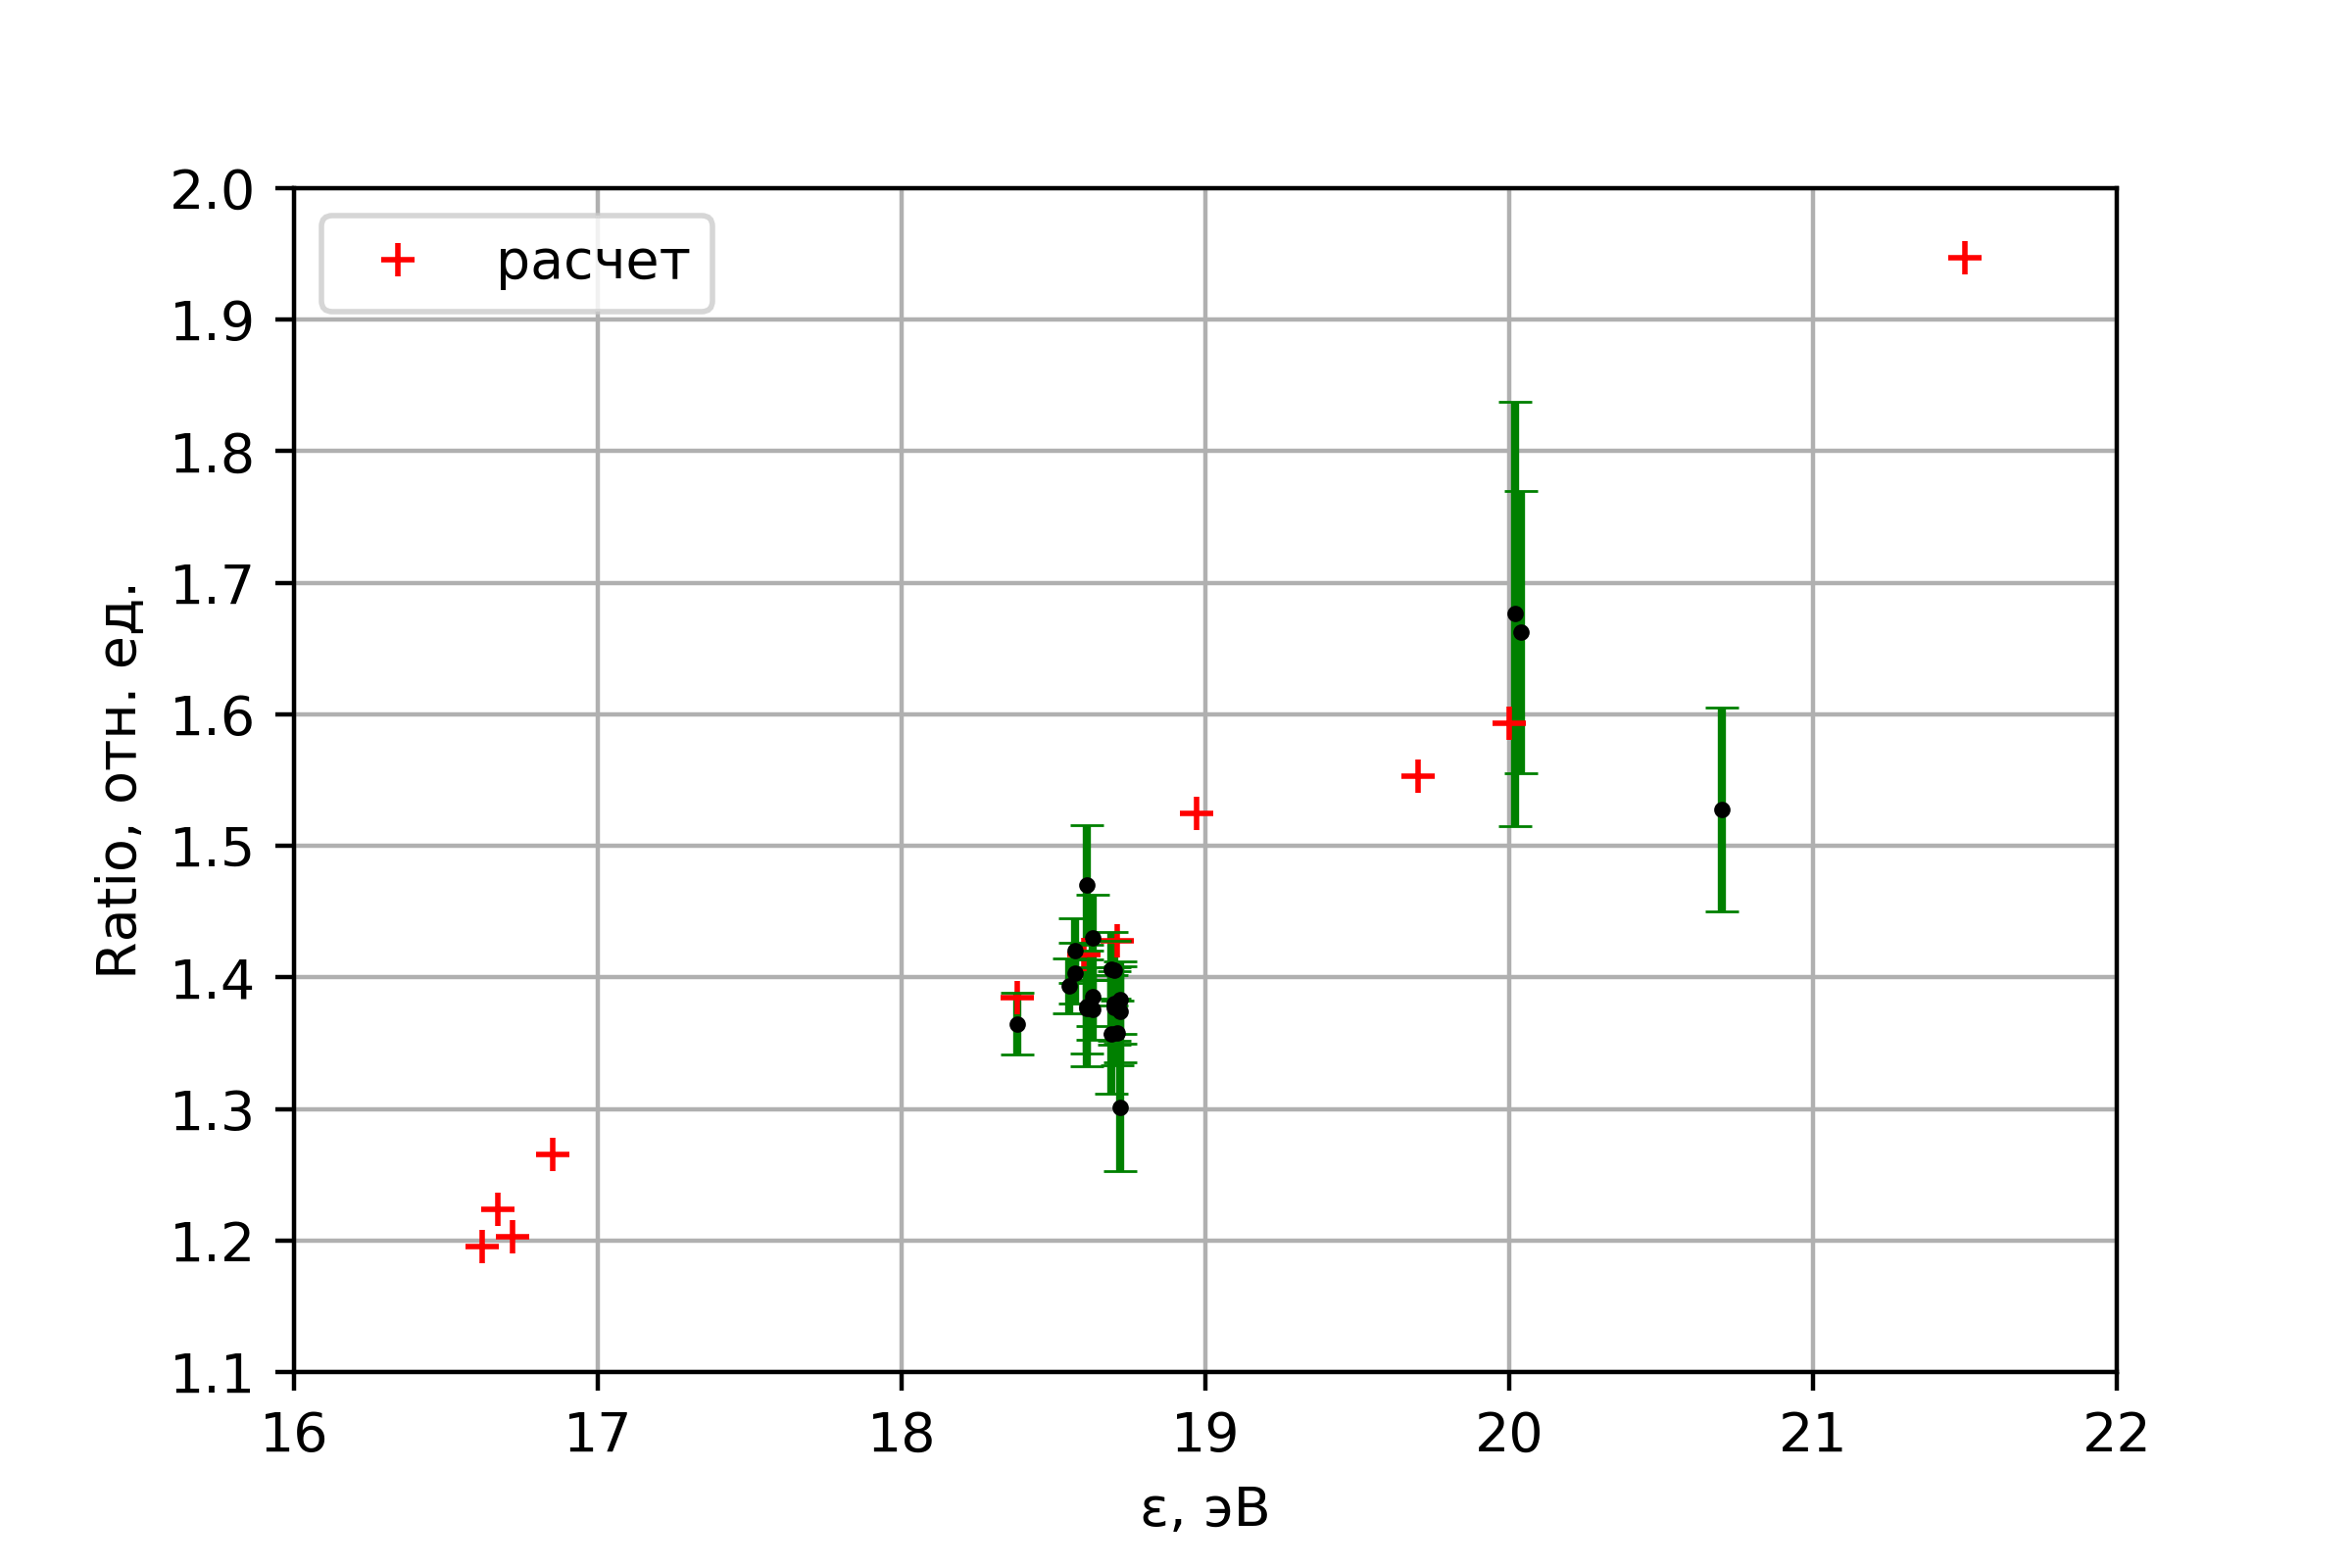
\includegraphics[width=16cm]{figures/Intensities_ratio}
  \caption{Зависимость ...... .}
  \label{fig:Intensities_ratio}
\end{figure}

Для оценки электронной температуры возмущенного пылевыми частицами положительного столба газового разряда постоянного
тока воспользуемся подходом, описанным в разделе \ref{sec:link_ratio_and_TE}. Для этого необходимо знать, как минимум,
параметры невозмущенного разряда: согласно [?..ссылка..?] осевое электрическое поле равняется $E_1 = 2.2$~В/см, а
электронная температура хвостовой части $T_e = 3.2$~эВ \cite{Zobnin2018}. Таким образом, на основе
(\ref{eq:intensities_ratio}) и полученных экспериментальных данных построим невязку $\eta$ с параметризацией значений
осевого электрического поля, которым задается предполагаемая ФРЭЭ возмущенного пылевым облаком газового разряда:
\begin{equation}
    \eta(E_2) = {1 \over N} \sum_{\forall \lambda \in experiment}{|R_{exp}(\lambda) - R_{calc}(\lambda, E_2)| \over {R_{exp}(\lambda) + R_{calc}(\lambda, E_2)}},
\end{equation}
где $E_2$~--~осевое электрическое поле возмущенного пылевыми частицами газового разряда, $R_{calc}$~--~расчетное
отношение интенсивностей, $R_{exp}$~--~отношение интенсивностей, полученное экспериментальным путем, $\lambda$~--~характеристики
спектральных линий, для которых найдено экспериментально отношение интенсивностей, N~--~кол-во таких спектральных линий.

Полученная невязка имеет четко выраженный минимум при осевом электрическом
поле $E_2 = 2.8$~В/см и значении невязки $\eta = 0.02$ (см.~рисунок~\ref{fig:discrepancy}).
При данном осевом электрическом поле, экспериментальные и расчетные отношения интенсивностей максимально близки друг другу,
что говорит о правильном подборе параметра $E_2$.
Совмещенные результаты экспериментальных отношений с расчетными можно посмотреть на рисунке \ref{fig:Intensities_ratio}.
Из данного графика видно, что расчетная модель довольно хорошо описывает эксперимент. Оценим электронную температуру
согласно (\ref{eq:Te_from_FRE}):



\backmatter %% Здесь заканчивается нумерованная часть документа и начинаются ссылки и
            %% заключение

\Conclusion % заключение к отчёту

В соответствии с поставленной научной задачей проведен обзор и отбор
экспериментальных данных Российско-европейского космического эксперимента
«Плазменный~кристалл~-~4». Отобранные экспериментальные данные включают в
себя: видеофайлы с обзорным изображением трубки газового разряда,
контролирующие распределение яркости свечения положительного столба и
положение плазменно-пылевого облака в положительном столбе, видеофайлы
высокого разрешения, характеризующие диаметр пылевого облака и концентрацию
пылевых частиц в нем, ток разряда и давление неона в газоразрядной камере,
сопутствующие спектры излучения положительного столба. Отобранные
эмиссионные спектры были обработаны с помощью специально разработанной
программой «Spectral Analyzer PK-4» с целью получения необходимой величины
отношения сигнал/шум. Получены отношения интенсивностей эмиссионных
спектральных линий неона, излучаемых положительным столбом с плазменно-пылевым
облаком и положительным столбом без пылевого облака. Показано, что
величина этого отношения зависит от энергии верхнего уровня соответствующего
энергетического перехода и варьируется от $1.4$ для уровней с энергий $18.5$~эВ до
$1.65$ для уровней с энергией $20$~эВ. Качественно очевидно, что такое увеличение
населенностей возбужденных уровней происходит вследствие увеличения
электронной температуры. Ввиду очень низкой плотности плазмы, количественный
анализ наблюдаемого эффекта проводился в рамках упрощенной модели заселения
возбужденных состояний прямым электронным ударом. Для определения
скоростей заселения возбужденных состояний функция распределения электронов
по энергиям определялась путем решения кинетического уравнения Больцмана для условий
данного эксперимента. Полученная функция имеет приблизительно «двухтемпературный» вид:
распределение электронов в диапазоне до $16$~эВ описывается
максвелловской функцией с температурой около $7$~эВ, в то время как в диапазоне
свыше $17$~эВ описывается максвелловской функцией с температурой около $3.5$~эВ,
что хорошо согласуется с литературными данными. Показано, что если взять за
исходную температуру «хвоста» электронной функции распределения
литературное значение $3.2$~эВ, то согласно предложенной методике и
спектральным данным в плазменно-пылевом облаке эта температура возрастет до
$3.5$~эВ. Таким образом, продемонстрирована возможность измерения температуры
«хвоста» функции распределения электронов на основе спектральных данных на
научной аппаратуре «Плазменный~кристалл~-~4».
\Acknowledgements %выражение благодарности
Автор выражает глубокую благодарность научному
руководителю Усачеву Александру Дмитриевичу за его безупречные знания и теплое отношение,
Зобнину Андрею Вячеславовичу за его помощь в составлении и решении
кинетического уравнения Больцмана, космонавту Олегу Дмитриевичу Кононенко за
выполнение эксперимента, а также международной научно-технической группе
«Плазменный~кристалл-4» (PK-4 Facility Science Team) за предоставленные
экспериментальные данные.

\nocite{*}
\bibliographystyle{gost780u}
\bibliography{0-main}


\appendix   % Тут идут приложения

\App
\label{app}

\section{Приложение А}
\label{app:app1}
Пример записи блока (одного спектра) в эксперименте. Спектральный файл обычно содержит более 1000 таких блоков, которые
следуют друг за другом.

\begin{small}
\begin{verbatim}
#########################################################################
# PK4 EAC SW -- Spectrometer
# started   2016-10-12'13:57:45.58 ~
# HPC=7679703032397 / HPCFreq=1496280000 Hz => HPC uptime = 5132.530698 s
# 2016-10-12'13:57:42.55; spectrometer commanded
# 2016-10-12'13:57:45.58; spectrometer response received
#--- spectrum ---
# 65535; spectrum start marker
#     0; data size flag
#     1; nr scans accumulated
#   750; integration time /ms
#     0; reserved value FPGA_ESV_MSW
# 12118; reserved value FPGA_ESV_LSW
#     0; pixel mode
   0:     0
   1:   471
   2:   484
   3:   466
   4:   510
   5:   506
   6:   484
   7:   451
   8:   491
   9:  1729
………..
………..
1022:   537
1023:   623
1024:   557
1025:   493
1026:   525
………..
………..
2038:   506
2039:   578
2040:   585
2041:   548
2042:   618
2043:   546
2044:   650
2045:   549
2046:   541
2047:   516
# 65533; spectrum end marker
#=== spectrum === read-out time = 2.172 s
# ended     2016-10-12'13:57:45.63 ~ (execution time = 0.051892 s)
# PK4 EAC SW -- Spectrometer
#########################################################################
\end{verbatim}
\end{small}

\section{Приложение Б}
\label{app:app2}
Пример записей логгера в эксперименте.

\begin{small}
\begin{verbatim}
Log Start: 04.06.2015 13:52:47
13:56:24 User and Reason: CADMOS OPS/CNES/PK4 commissioning
13:56:24 Opening Parameter File
13:56:26 readParameterFile: Read 1576 key-value-pairs from Parameter File
13:56:28 setOpMode: Detected IBP actual machine state OP_PUMPING.
...      Requesting for new machine state OP_MINIMAL.
13:56:28 checkMod01Operative: Starting to check if Module 02-Power
...      is operative
13:56:31 M01_temperature_cm01 measured 27.100 expected 30 abs-diff 2.900
...      ranges -20 +20 all [°C] result: ok
13:56:31 M01_Vin_M02_off measured 23.975 expected 24 abs-diff 0.025
...      ranges -2 +1.5 all [V] result: ok
13:56:32 M01_Vout_M02_off measured 0.000 expected 0 abs-diff 0.000
...      ranges -0 +0.1 all [V] result: ok
13:56:32 M01_current_M02_off measured 0.001 expected 0.002 abs-diff 0.001
...      ranges -0.002 +0.002 all [A] result: ok
13:56:32 M01_Vin_M03_off measured 23.950 expected 24 abs-diff 0.050 ranges
...      -2 +1.5 all [V] result: ok
13:56:32 M01_Vout_M03_off measured 0.000 expected 0 abs-diff 0.000 ranges
...      -0 +0.1 all [V] result: ok
13:56:32 M01_current_M03_off measured 0.001 expected 0.002 abs-diff 0.001
...      ranges -0.002 +0.002 all [A] result: ok
13:56:32 M01_Vin_M04_off measured 23.975 expected 24 abs-diff 0.025 ranges
...      -2 +1.5 all [V] result: ok
………..
………..

15:25:04 TrapAndManipulate : begin flushing
15:25:04 setFlushing: Flushing with 10sccm for 10 seconds
15:25:04 setIQF200GasFlow: Changing IQF200 Gasflow to 10sccm.
15:25:04 setIQF200ValveMode: Changing ValveMode to 2
15:25:14 setIQF200GasFlow: Changing IQF200 Gasflow
...      to 0.0231250002980232sccm.
15:25:14 setIQF200ValveMode: Changing ValveMode to 2
15:25:14 TrapAndManipulate : end flushing
15:25:14 TrapAndManipulate : standby with gasflow 0.5 sccm for 10 s
15:25:14 setIQF200GasFlow: Changing IQF200 Gasflow to 0.5sccm.
15:25:14 setIQF200ValveMode: Changing ValveMode to 2
15:25:26 *** end trapping ***
15:25:26 *** GasJet 3 Dispenser setting cycle 6 ***
15:25:26 setIQP600Pressure: old IQP600 pressure is 300mbar.
...      Trying to set 300mbar
15:25:26 setGRValveMode : duration for sending open command:
...      5.01350212097168
15:25:26 setGRValveMode: Changing GR-ValveMode to 0
………..
………..
17:11:51 saveChamberEvacuation: Finished with evacuating Chamber
17:11:52 setGRValveMode : duration for sending open command:
...      5.21663045883179
17:11:53 setGRValveMode: Opened GR Valve. Module 07 Current
...      (before/300ms after opening): 177 176
17:11:53 setGRValveMode: Changing GR-ValveMode to 1
17:11:53 saveGREvacuation: Finished with evacuating GR
17:11:53 restorePumpingMode: Finished with restoring mode OP_PUMPING
17:11:53 Finished, Exception was: Script TERMINATED by USER
Log End: 04.06.2015 17:25:30
\end{verbatim}
\end{small}


\end{document}
